\documentclass{article}

\usepackage{amsmath}
\usepackage[letterpaper, margin=1in, footskip=.25in]{geometry}
\usepackage{fancyhdr}
\usepackage{lipsum}
\usepackage{graphicx}
\usepackage{subcaption}
\usepackage{wrapfig}
\usepackage[hidelinks]{hyperref}
\usepackage{xcolor}
\usepackage[nottoc,notlof,notlot,numbib]{tocbibind}

\title{Volumes of Parabola-Line Solids of Revolution}
\author{Steven Labalme}
\date{\today}

\begin{document}

\maketitle
\pagenumbering{gobble}
\newpage
\tableofcontents
\listoffigures
\pagenumbering{roman}
\newpage

\pagestyle{fancy}
\fancyhf{}
\rfoot{Labalme \thepage}
\renewcommand{\headrulewidth}{0pt}
\pagenumbering{arabic}
\setcounter{secnumdepth}{0}

\begin{center}
\section{Abstract}
\end{center}
\begin{figure}[h!]
  \centering
  \begin{subfigure}[b]{0.4\linewidth}
    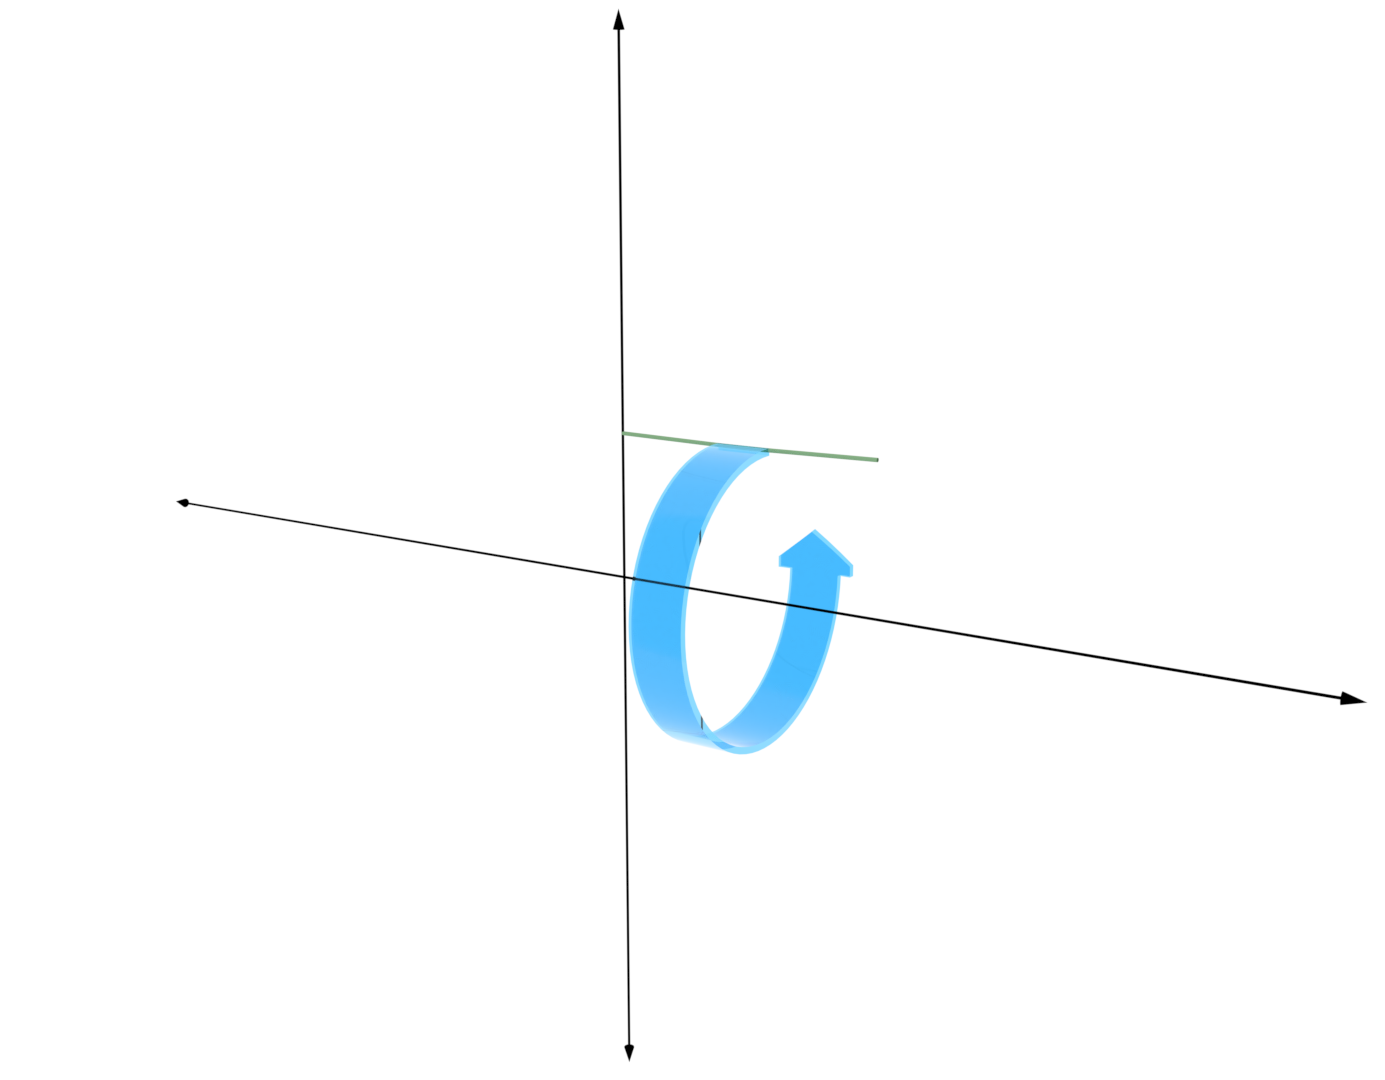
\includegraphics[width=\linewidth]{Blender/ParabolaLineIntegration-AbstractCylinder-f_0001.png}
    \caption{Cylinder.}
    \label{fig:abstracta}
  \end{subfigure}
  \begin{subfigure}[b]{0.4\linewidth}
    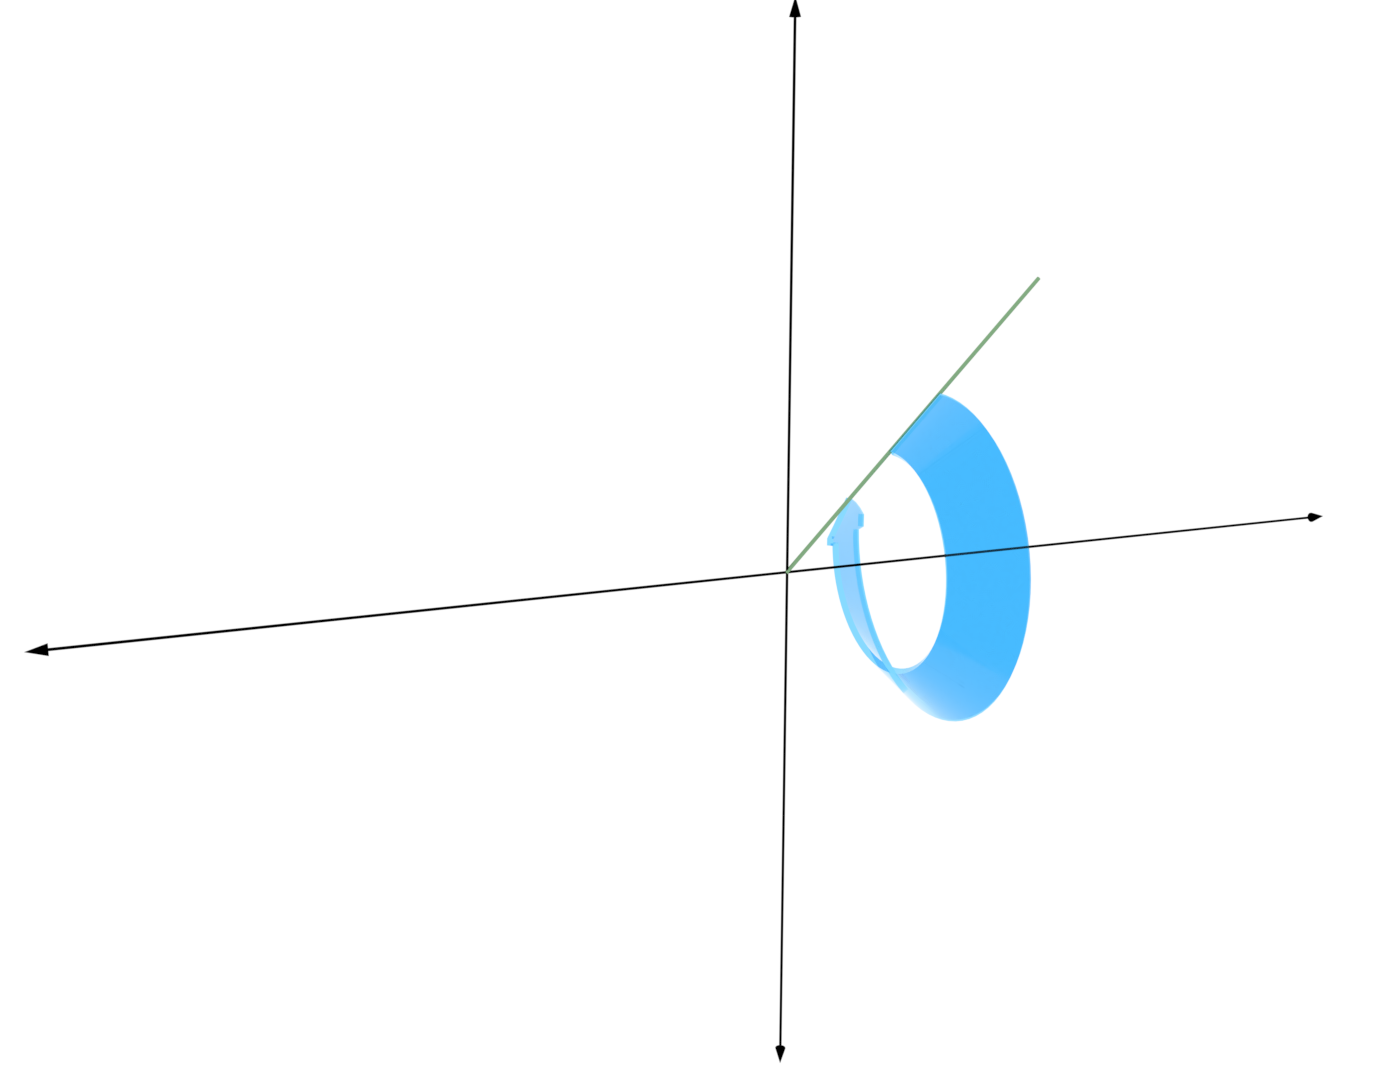
\includegraphics[width=\linewidth]{Blender/ParabolaLineIntegration-AbstractCone-f_0001.png}
    \caption{Cone.}
    \label{fig:abstractb}
  \end{subfigure}
  \caption{Solids of revolution.}
  \label{fig:abstract}
\end{figure}
A solid of revolution is a three-dimensional geometric figure created by rotating a curve around an axis over a certain distance. Solids of revolution are identifiable by the fact that a cross-section perpendicular to the axis will be, at any point along the height of the solid, a circle. Some simple solids of revolution are the cylinder (created by rotating a line --- such as $y=1$ --- about an axis parallel to the initial line --- such as $y=0$ --- over an interval --- such as $[0,2]$ --- as seen in Figure \ref{fig:abstracta}) and the cone (created by rotating a line --- such as $y=x$ --- about an axis that is not parallel to the initial line --- such as $y=0$ --- over an interval --- such as $[0,2]$ --- as seen in Figure \ref{fig:abstractb}). The volume of the type of solid of revolution pictured in Figure \ref{fig:abstract} (that is, one that rotates about the x or y-axis) is fairly easy to find. For instance, if we imagine a circle passing along the x-axis in Figure \ref{fig:abstractb} with variable radius, $f(x)$, its area at point, $(x,f(x))$, is $A=\pi x^2$. Integrating over $[0,x]$ gives the more familiar $V=\frac{1}{3}\pi x^3$. However, the volume of a solid of revolution whose axis is not the x or y-axis is far more difficult to find.
\begin{figure}[h!]
  \centering
  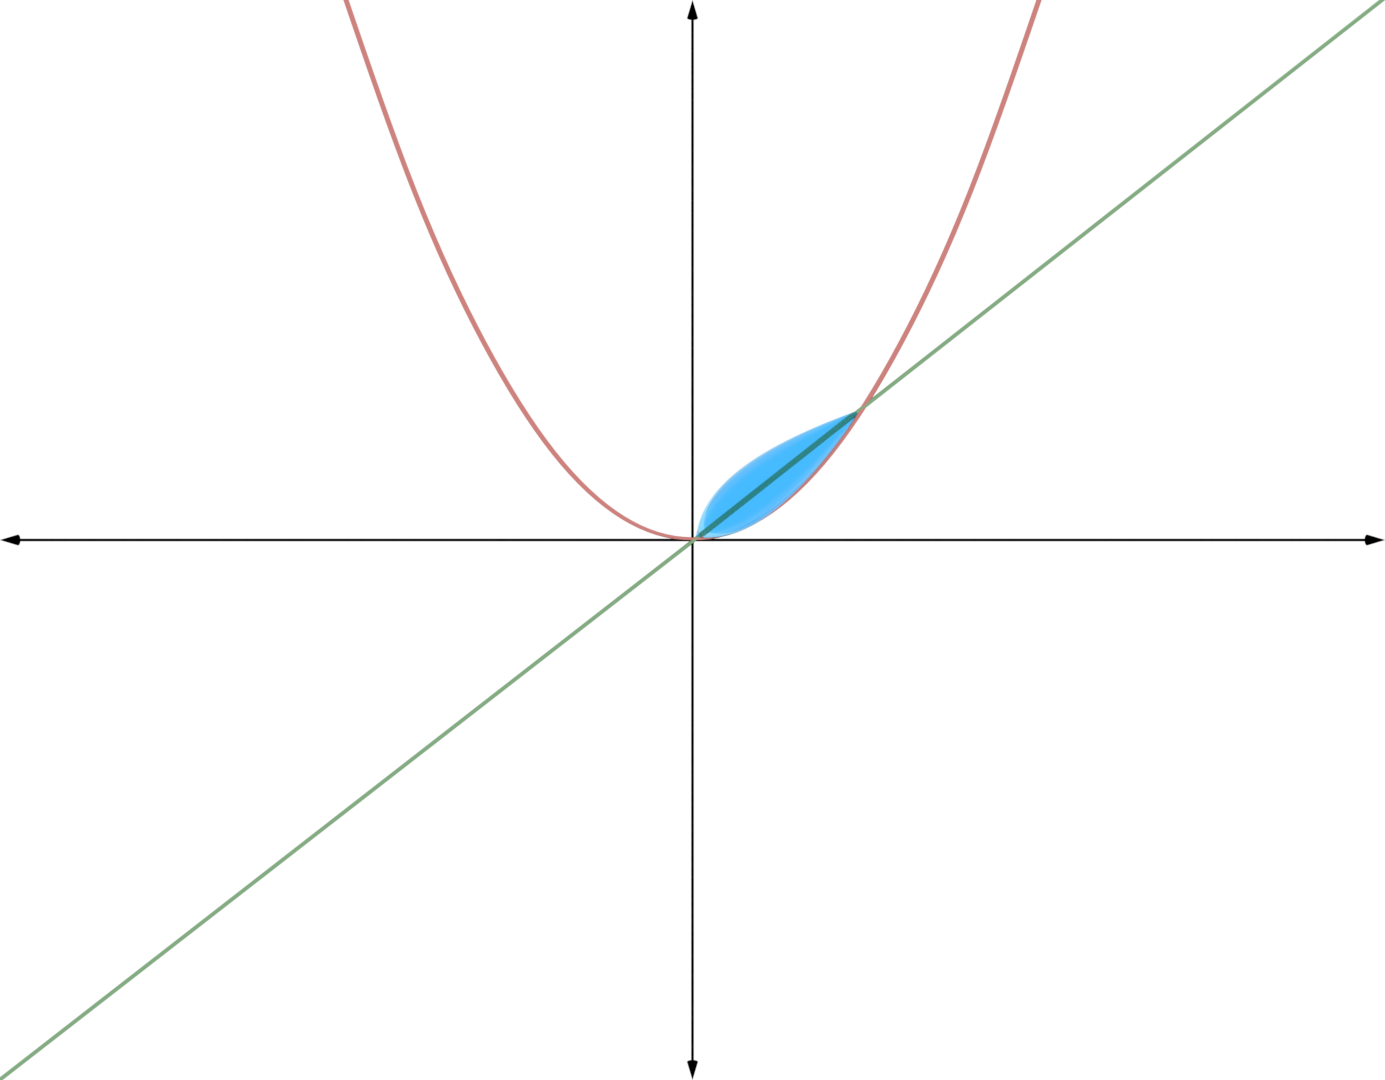
\includegraphics[width=0.6\linewidth]{Blender/ParabolaLineIntegration-AbstractTeardrop-f_0090.png}
  \caption{Teardrop-shaped solid of revolution.}
  \label{fig:abstract2}
\end{figure}\par
The purpose of this paper is to determine the volume of the class of solids of revolution created by rotating the parabola, $y=ax^2$, about the axis, $y=bx$ where both $a$ and $b$ are positive, real numbers. This class of solids all exhibit a similar, teardrop-like appearance, as seen in Figure \ref{fig:abstract2}. The assignment was to use three different methods to analyze these shapes (one per section).\par
The conclusion of each section was identical. Every method supports the hypothesis that the volume of this class of solids of revolution as a function of $a$ and $b$ is given by$$V=\frac{\pi b^5}{30a^3\sqrt{1+b^2}}$$
\newpage

\setcounter{secnumdepth}{3}

\section{Cone Method}
\subsection{Introduction}
\begin{figure}[h!]
  \centering
  \begin{subfigure}[b]{0.4\linewidth}
    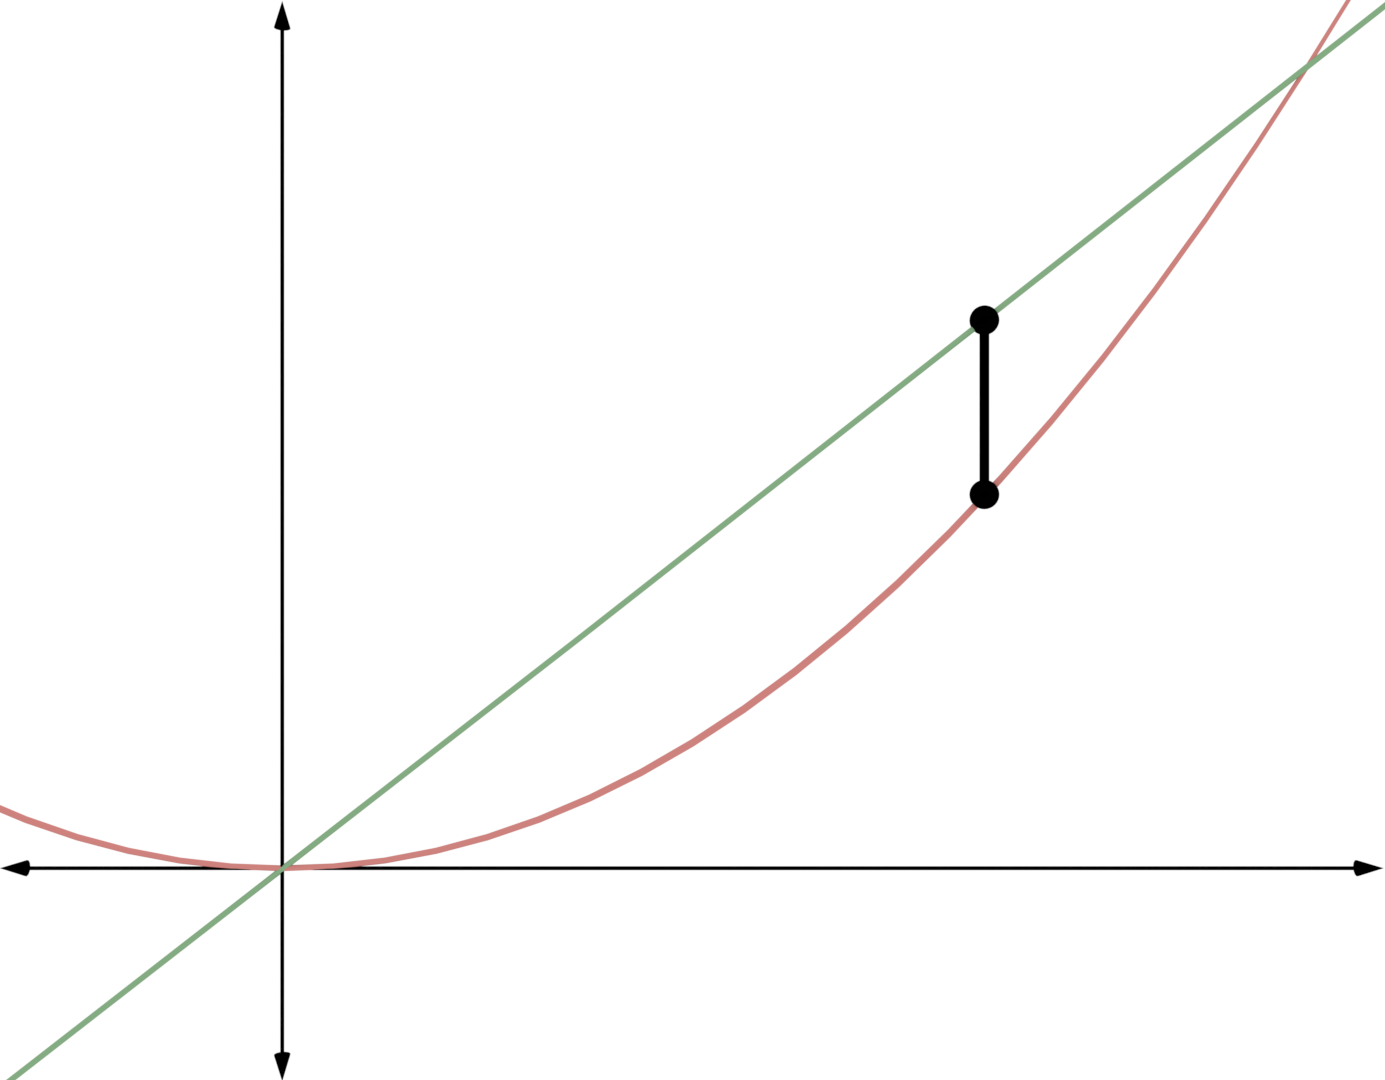
\includegraphics[width=\linewidth]{Blender/ParabolaLineIntegration-ConeDiagram-f2_0001.png}
    \caption{Line to be rotated.}
    \label{fig:conea}
  \end{subfigure}
  \begin{subfigure}[b]{0.4\linewidth}
    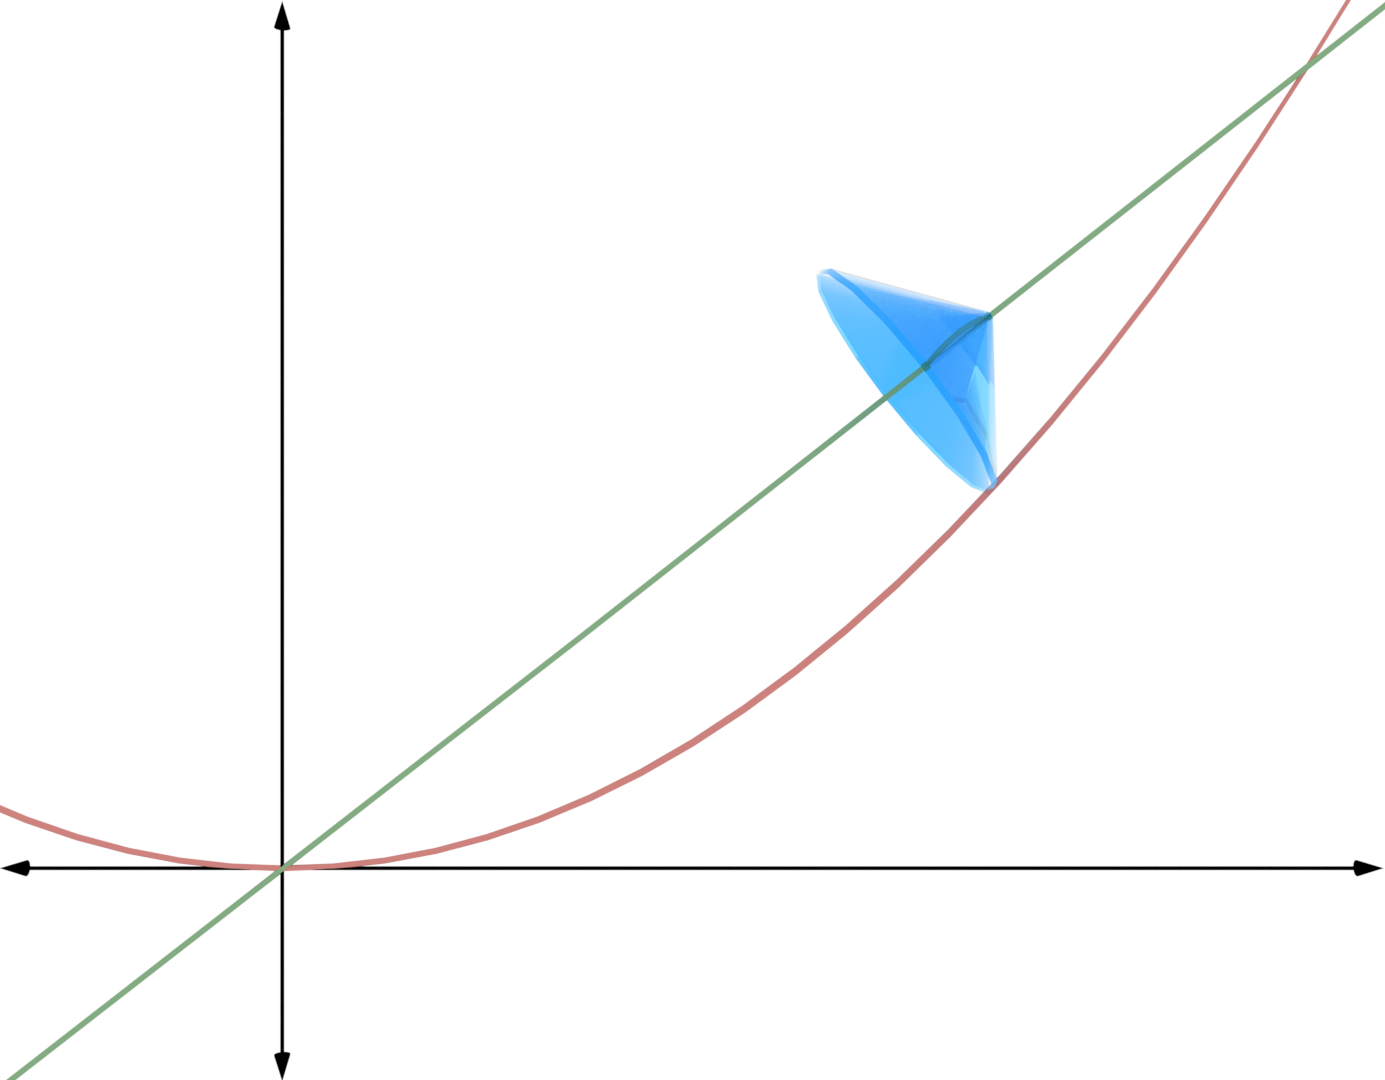
\includegraphics[width=\linewidth]{Blender/ParabolaLineIntegration-ConeGIF-f2_0090.png}
    \caption{Cone of rotation.}
    \label{fig:coneb}
  \end{subfigure}
  \caption{Formation of the cone of revolution.}
  \label{fig:cone}
\end{figure}

Even though the shell and disk methods are the most widely taught techniques\footnote{\label{fot:1}At the AP BC Calculus level.} of using integral calculus to find volume (using cylindrical and circular approximations, respectively), the most algebraically simple method of approximating the volume of the teardrop-shaped solid of revolution formed by rotating $y=ax^2$ around the axis, $y=bx$, uses cones.\par
First, it involves constructing a vertical line segment down from the axis, $y=bx$, to the parabola, $y=ax^2$, as seen in Figure \ref{fig:conea}. This segment is rotated around the axis to form a cone with no base, as seen in Figure \ref{fig:coneb}. Once the lateral area of this cone is found as a function of $x$ (it is the lateral area that approximates the volume), this function is integrated from 0 to the rightmost intersection of the axis and the parabola.

\subsection{Derivation} \label{deriv1}
\paragraph{THEOREM} The volume of the solid of revolution created by rotating the parabola, $y=ax^2$, about the line, $y=bx$, is $\frac{\pi b^5}{30a^3\sqrt{1+b^2}}$ where $a>0$ and $b>0$.\par
\smallskip
\paragraph{PROOF} Begin by finding the distance between $y=bx$ and $y=ax^2$ as a function of $x$. Use the distance formula,$$d=\sqrt{\left(x_2-x_1\right)^2+\left(y_2-y_1\right)^2}$$with $x$ plugged in for $x_1$ and $x_2$, $bx$ for $y_2$, and $ax^2$ for $y_1$. This gives$$\ell=\sqrt{\left(x-x\right)^2+\left(bx-ax^2\right)^2}$$ which can be simplified as follows. Note that $\ell$ is substituted for $d$ because the distance given by the formula is the slant height of the cone of rotation.
\begin{align*}
\ell &=\sqrt{\left(x-x\right)^2+\left(bx-ax^2\right)^2}\\
      &=\sqrt{\left(0\right)^2+\left(bx-ax^2\right)^2}\\
      &=\sqrt{\left(bx-ax^2\right)^2}\\
      &=bx-ax^2\tag{1}
\end{align*}\par
\begin{figure}[t]
  \centering
  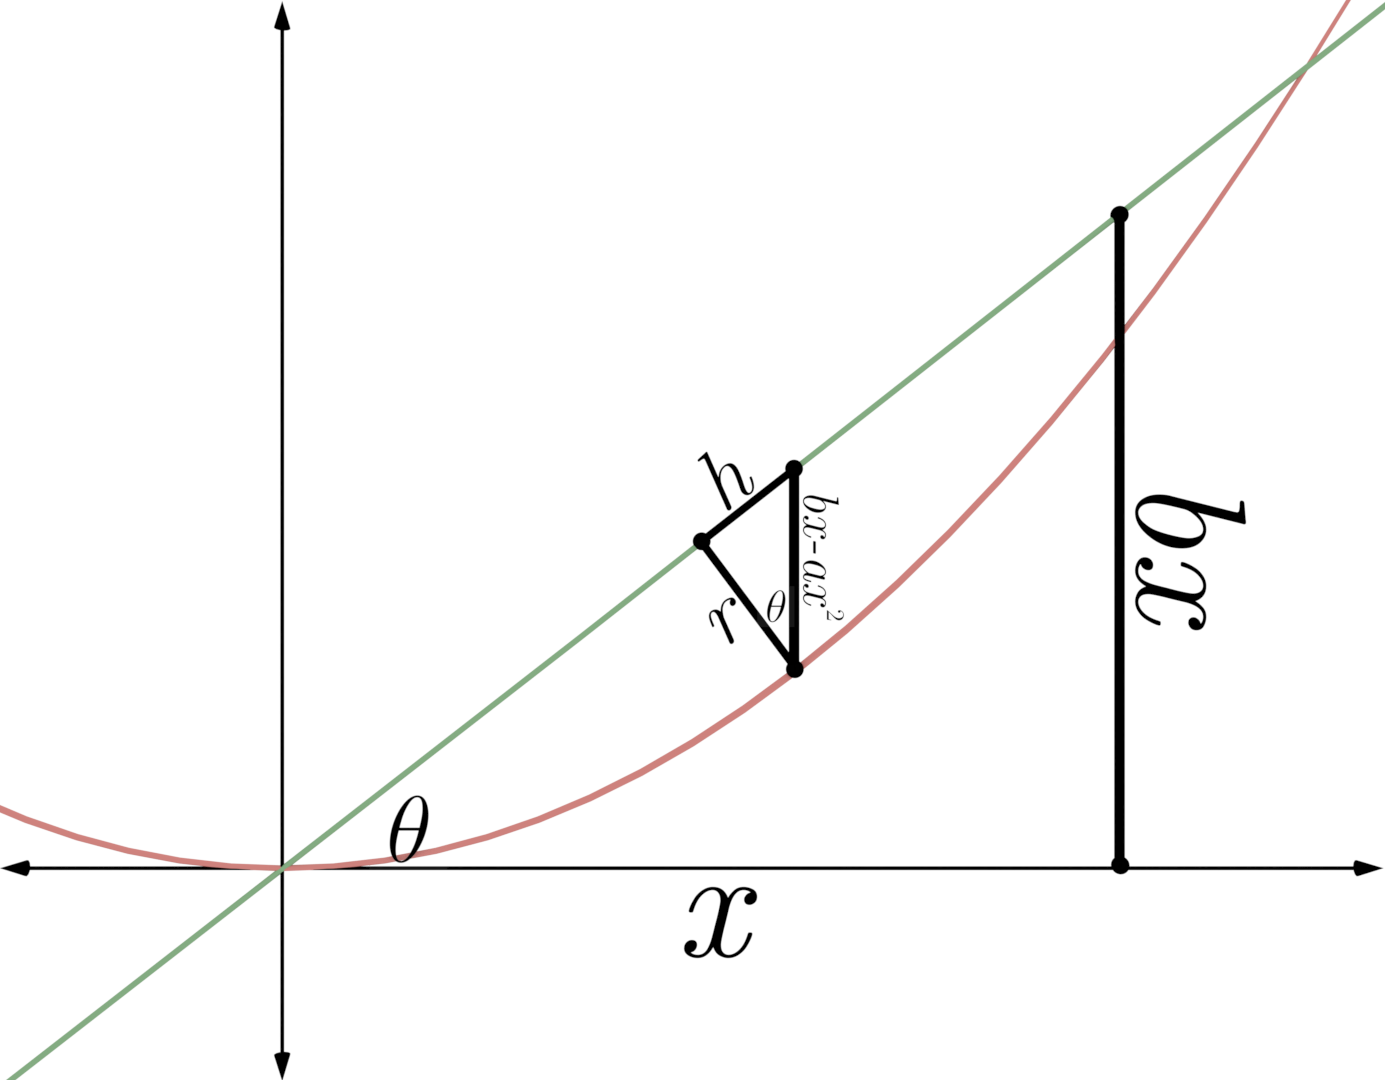
\includegraphics[width=0.6\linewidth]{Blender/ParabolaLineIntegration-ConeTriangles-f2_0001.png}
  \caption{Derivation of the radius as a function of $x$.}
  \label{fig:cone2}
\end{figure}
Next, find the radius of the cone as a function of $x$. In Figure \ref{fig:cone2}, a right triangle is constructed within the cone --- $bx-ax^2$ is the hypotenuse, and the height, $h$, and radius, $r$, are unknown. Theta, $\theta$, is in the bottom, left hand corner of the triangle and is equal to $\theta$ near the origin. Additionally, in Figure \ref{fig:cone2}, there is a second triangle with legs\footnote{By the substitution $y=bx$.} $x$ and $bx$ that allows us to find $\theta$ as a function of $b$.\par
The definition of tangent gives the following equation. Simplify, and solve for $\theta$.
\begin{align*}
\tan\theta &=\frac{bx}{x}=b\\
\theta       &= \tan^{-1}\left(b\right)
\end{align*}
\begin{wrapfigure}[12]{l}{0.5\textwidth}
  \centering
  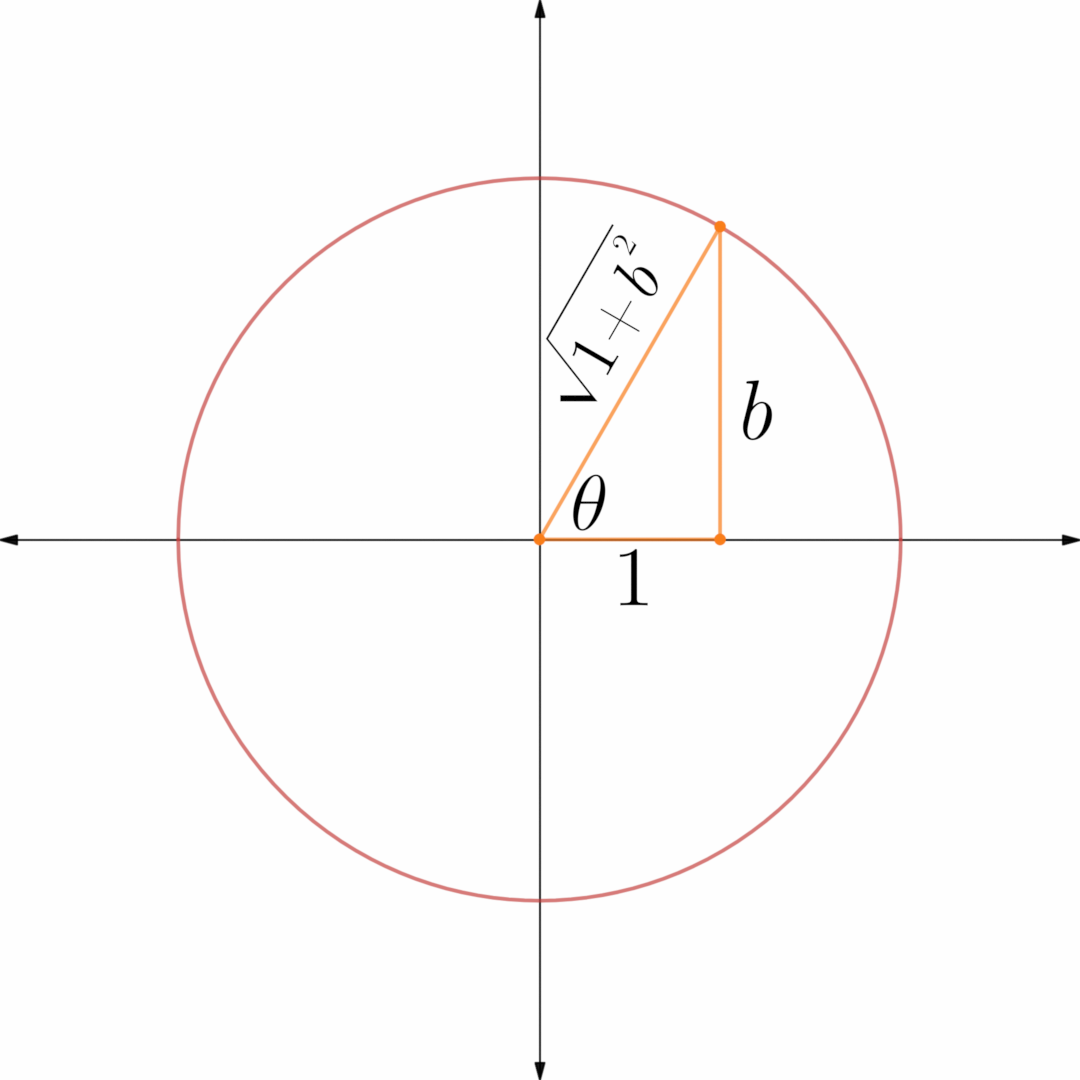
\includegraphics[width=0.47\textwidth]{Blender/ParabolaLineIntegration-ConeTanTriangle-f2_0001.png}
  \caption{\label{fig:cone3}Simplification of $\cos\left(\tan^{-1}\left(b\right)\right)$.}
\end{wrapfigure}
The definition of cosine gives the following equation. Simplify, and solve for $r$. For a visualization of why $\cos\left(\tan^{-1}\left(b\right)\right)$ simplifies, refer to Figure \ref{fig:cone3}.
\begin{align*}
\frac{r}{bx-ax^2} &=\cos\theta\\
                           &=\cos\left(\tan^{-1}\left(b\right)\right)\\
                           &=\frac{1}{\sqrt{1+b^2}}\\
r                          &=\frac{bx-ax^2}{\sqrt{1+b^2}}\tag{2}
\end{align*}
Equipped with functions for both the slant height and radius of the cone of rotation (equations 1 and 2, respectively), plug into the lateral area formula.
\begin{align*}
LA &=\pi r\ell\\
     &=\pi\left(\frac{bx-ax^2}{\sqrt{1+b^2}}\right)\left(bx-ax^2\right)\\
     &=\frac{\pi\left(bx-ax^2\right)^2}{\sqrt{1+b^2}}\tag{3}
\end{align*}\par
Integrate equation 3 from 0 to the rightmost intersection of $y=ax^2$ and $y=bx$ (an interval on which the cones' dimensions are real) with respect to $x$.\par
First, it is necessary to derive this rightmost intersection as a function of $a$ and $b$. Set the two equations equal to each other to give$$ax^2=bx$$which can be reordered to give$$ax^2-bx=0$$which can be factored to give$$\left(x\right)\left(ax-b\right)=0$$\par
According to the Zero Product Property, the two intersections are at $x=0$ and $ax-b=0$ (or $x=\tfrac{b}{a}$). Therefore, we must integrate on the interval, $\left[0,\tfrac{b}{a}\right]$. The volume equation is$$V=\int_0^{\frac{b}{a}}\frac{\pi\left(bx-ax^2\right)^2}{\sqrt{1+b^2}}dx$$which can be simplified as follows.
\begin{align*}
V &= \int_0^{\frac{b}{a}}\frac{\pi\left(bx-ax^2\right)^2}{\sqrt{1+b^2}}dx\\
   &= \frac{\pi}{\sqrt{1+b^2}}\int_0^{\frac{b}{a}}\left(bx-ax^2\right)^2dx\\
   &= \frac{\pi}{\sqrt{1+b^2}}\int_0^{\frac{b}{a}}b^2x^2-2abx^3+a^2x^4dx\\
   &= \frac{\pi}{\sqrt{1+b^2}}\left(\int_0^{\frac{b}{a}}b^2x^2dx-\int_0^{\frac{b}{a}}2abx^3dx+\int_0^{\frac{b}{a}}a^2x^4dx\right)\\
   &= \frac{\pi}{\sqrt{1+b^2}}\left(b^2\int_0^{\frac{b}{a}}x^2dx-2ab\int_0^{\frac{b}{a}}x^3dx+a^2\int_0^{\frac{b}{a}}x^4dx\right)\\
   &= \frac{\pi}{\sqrt{1+b^2}}\left(b^2\left[\frac{x^3}{3}\right]_0^{\frac{b}{a}}-2ab\left[\frac{x^4}{4}\right]_0^{\frac{b}{a}}+a^2\left[\frac{x^5}{5}\right]_0^{\frac{b}{a}}\right)\\
   &= \frac{\pi}{\sqrt{1+b^2}}\left(b^2\left[\frac{\frac{b}{a}^3}{3}-\frac{0^3}{3}\right]-2ab\left[\frac{\frac{b}{a}^4}{4}-\frac{0^4}{4}\right]+a^2\left[\frac{\frac{b}{a}^5}{5}-\frac{0^5}{5}\right]\right)\\
   &= \frac{\pi}{\sqrt{1+b^2}}\left(b^2\left[\frac{b^3}{3a^3}\right]-2ab\left[\frac{b^4}{4a^4}\right]+a^2\left[\frac{b^5}{5a^5}\right]\right)\\
   &= \frac{\pi}{\sqrt{1+b^2}}\left(\frac{b^5}{3a^3}-\frac{b^5}{2a^3}+\frac{b^5}{5a^3}\right)\\
   &= \frac{\pi}{\sqrt{1+b^2}}\left(\frac{10b^5}{30a^3}-\frac{15b^5}{30a^3}+\frac{6b^5}{30a^3}\right)\\
   &= \frac{\pi}{\sqrt{1+b^2}}\left(\frac{b^5}{30a^3}\right)\\
   &= \frac{\pi b^5}{30a^3\sqrt{1+b^2}}\tag{4}
\end{align*}\par
\begin{flushright}
\textbf{Q.E.D.}
\end{flushright}

\subsection{Summary}
The approximation of the volume of the solids of revolution created by rotating the parabola, $y=ax^2$, about the line, $y=bx$, by way of cones is the least mathematically complicated of the methods listed in this paper. I was introduced to it by DavidK of Mathematics Stack Exchange in his answer \cite{BIB:cone} to my related question \cite{BIB:disk2}. It requires only a beginner's knowledge of trigonometry, no major algebraic derivations, and a relatively quick calculus step that relies on the reverse power rule, alone, after the factoring of constants. However, despite the rather straightforward approach, using cones to approximate volume is not commonly taught (see Footnote \ref{fot:1}), so this method can take some time to develop that the following techniques do not.\par
The next method is the next simplest --- it is a variation of the Shell Method.
\newpage

\section{Shell Method}
\subsection{Introduction}

\begin{figure}[h!]
  \centering
  \begin{subfigure}[b]{0.32\linewidth}
    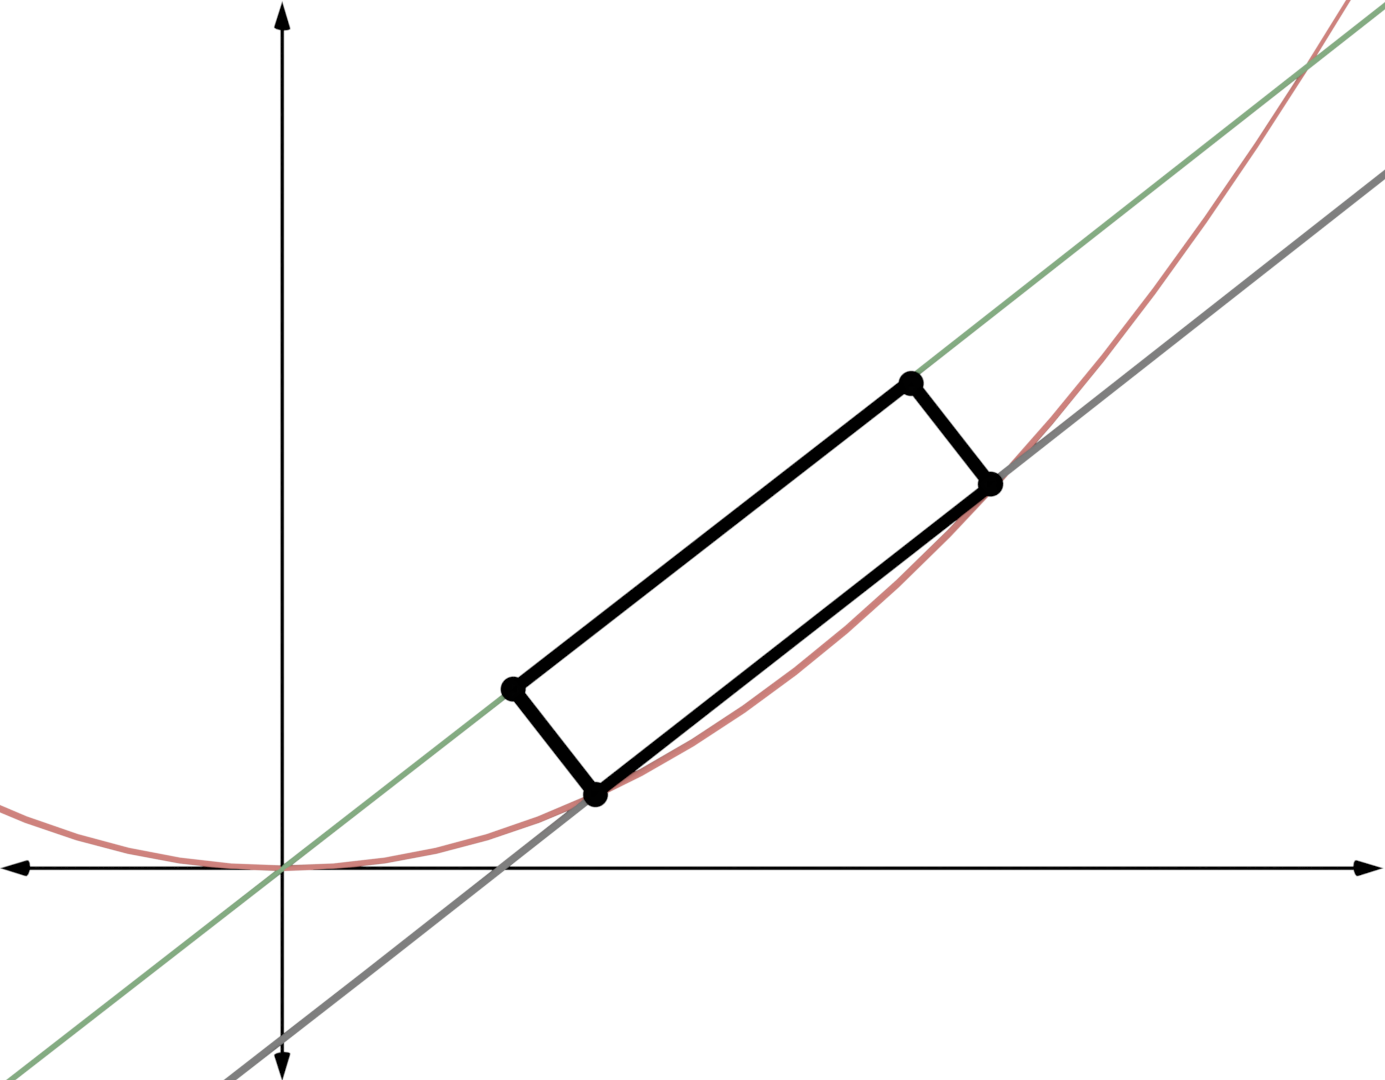
\includegraphics[width=\linewidth]{Blender/ParabolaLineIntegration-ShellDiagram-f2_0001.png}
    \caption{Rectangle and $y=bx+c$.}
    \label{fig:shella}
  \end{subfigure}
  \begin{subfigure}[b]{0.32\linewidth}
    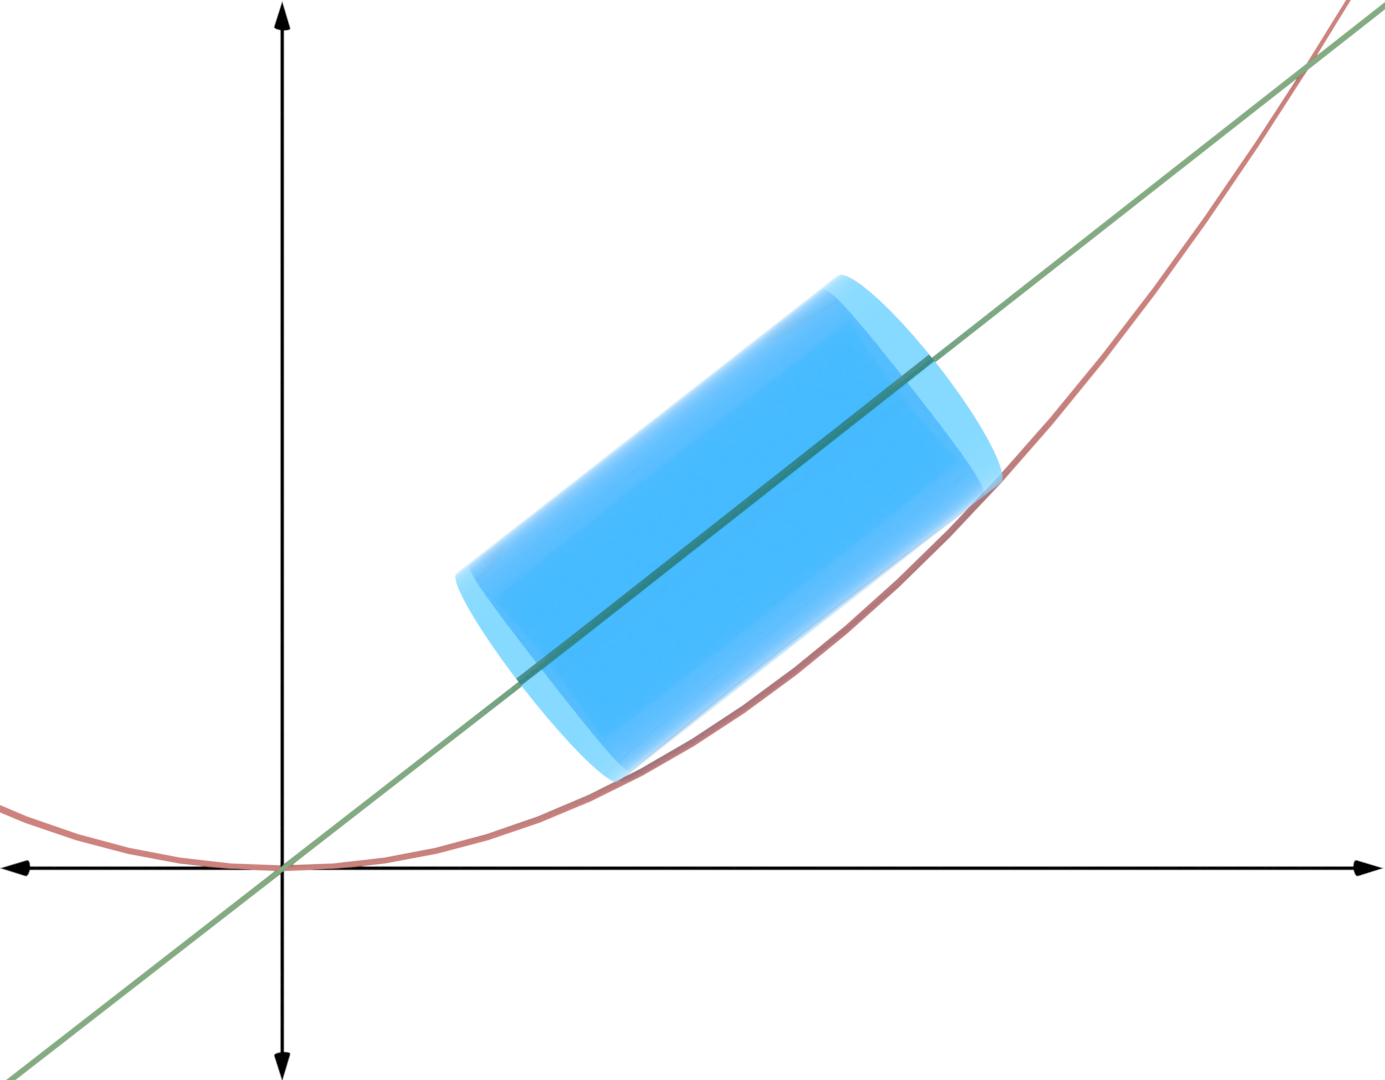
\includegraphics[width=\linewidth]{Blender/ParabolaLineIntegration-ShellCylinder1-f2_0001.png}
    \caption{Shell from previous rectangle.}
    \label{fig:shellb}
  \end{subfigure}
  \begin{subfigure}[b]{0.32\linewidth}
    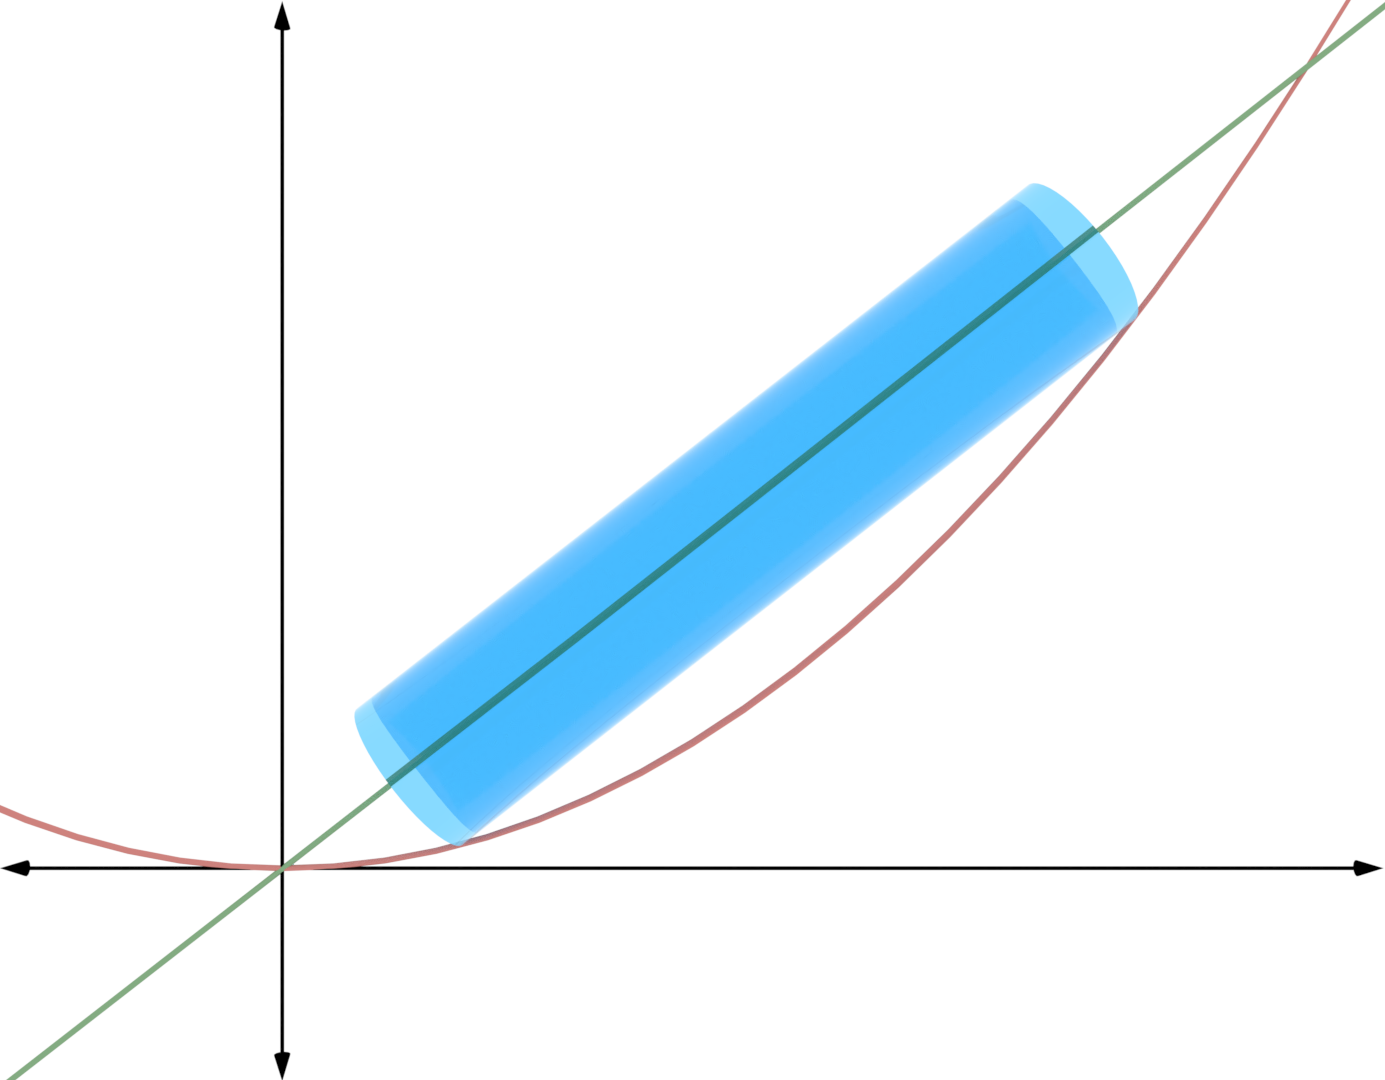
\includegraphics[width=\linewidth]{Blender/ParabolaLineIntegration-ShellCylinder2-f2_0001.png}
    \caption{A different shell.}
    \label{fig:shellc}
  \end{subfigure}
  \caption{Formation of the shells.}
  \label{fig:shell1}
\end{figure}

This is the first of the two commonly taught methods of integrating to find volume. It utilizes a rectangle extended from the axis, $y=bx$, with sufficient length and position to evenly touch two points along the parabola, $y=ax^2$, that are of the same distance from the axis, as seen in Figure \ref{fig:shella}. This rectangle is then spun around the axis to create a cylinder within the initial teardrop shape (see Figure \ref{fig:abstract2}), as seen in Figure \ref{fig:shellb}. It is the lateral area of the cylinder that is, once again, used to approximate the volume. While cylindrical shells generally increase in radius from the center to the edge of the solid of revolution with height, $f(x)$, the shells necessary for this problem begin with their maximum radius and minimum height, and as the radius decreases, the height increases to reach out to further and further points of the teardrop shape, as seen in the progression from Figure \ref{fig:shellb} to Figure \ref{fig:shellc}.\par
This method requires more initial algebra to generate the eventual integrable equation. First, construct a line, $y=bx+c$, parallel to the axis where $c$ is a constant (the grey line in Figure \ref{fig:shella}). This line, within the right range, will intersect between one and two points on $y=ax^2$ that are equidistant from the axis. The distance between these points (the height of the shell as a function of $c$) is easy to solve for. Then, trigonometry gives the radius as a function of $c$. Finally, determine the interval on which $c$ can realistically vary, and integrate.

\subsection{Derivation} \label{deriv2}
\paragraph{THEOREM} The volume of the solid of revolution created by rotating the parabola, $y=ax^2$, about the line, $y=bx$, is $\frac{\pi b^5}{30a^3\sqrt{1+b^2}}$ where $a>0$ and $b>0$.\par
\smallskip
\paragraph{PROOF} Begin by constructing a line, $y=bx+c$ parallel to $y=bx$ and a vertical distance $c$ from it (the grey line in Figure \ref{fig:shella}). Next, find the distance between the two lines --- imagine a perpendicular to $y=bx$ that passes through both lines, and the goal is to find the distance between the two points of intersection. This will be the radius of the shell as a function of $c$.\par
The determination of the radius, $r$, is almost identical to the related procedure in section \ref{deriv1}, except for two things. First, the small triangle in Figure \ref{fig:cone2} is wedged between the axis and the grey line instead of the axis and the parabola. Second, the hypotenuse of said triangle is given ($c$) and does not need to be derived ($bx-ax^2$). Still, a refresher follows to introduce the new variables (refer to Figures \ref{fig:cone2} and \ref{fig:cone3} for related visuals).\par
The definition of tangent gives the following equation. Simplify, and solve for $\theta$.
\begin{align*}
\tan\theta &=\frac{bx}{x}=b\\
\theta       &= \tan^{-1}\left(b\right)
\end{align*}
The definition of cosine gives the following equation. Simplify, and solve for $r$. For a visualization of why $\cos\left(\tan^{-1}\left(b\right)\right)$ simplifies, refer to Figure \ref{fig:cone3}. Note that the absolute value of $c$ is taken because the radius is always a positive quantity.
\begin{align*}
\frac{r}{|c|} &=\cos\theta\\
                           &=\cos\left(\tan^{-1}\left(b\right)\right)\\
                           &=\frac{1}{\sqrt{1+b^2}}\\
r                          &=\frac{|c|}{\sqrt{1+b^2}}\tag{5}
\end{align*}\par
Next, find the height, $h$, of a shell as a function of $c$. To do this, find the distance between the two points, $\left(x_1,y_1\right)$ and $\left(x_2,y_2\right)$, where $y=bx+c$ intersects the parabola, $y=ax^2$, as seen in Figure \ref{fig:shell2}.\par
Set $y=bx+c$ equal to $y=ax^2$ and solve for $x$, as follows. The two solutions to the quadratic formula are $x_1$ and $x_2$.
\begin{align*}
bx+c &= ax^2\\
0 &= ax^2-bx-c\\
x &= \frac{-(-b)\pm\sqrt{(-b)^2-4(a)(-c)}}{2(a)}\\
   &= \frac{b\pm\sqrt{b^2+4ac}}{2a}\\
\end{align*}
\vspace{-2em}
\begin{align*}
x_1 &= \frac{b-\sqrt{b^2+4ac}}{2a} &
x_2 &= \frac{b+\sqrt{b^2+4ac}}{2a}
\end{align*}\par
Variables $y_1$ and $y_2$ can be found by plugging $x_1$ and $x_2$ into $y=bx+c$. Therefore, they are as follows.
\begin{align*}
y_1 &= \frac{b^2+2ac-b\sqrt{b^2+4ac}}{2a} &
y_2 &= \frac{b^2+2ac+b\sqrt{b^2+4ac}}{2a}
\end{align*}
\begin{figure}[h!]
  \centering
  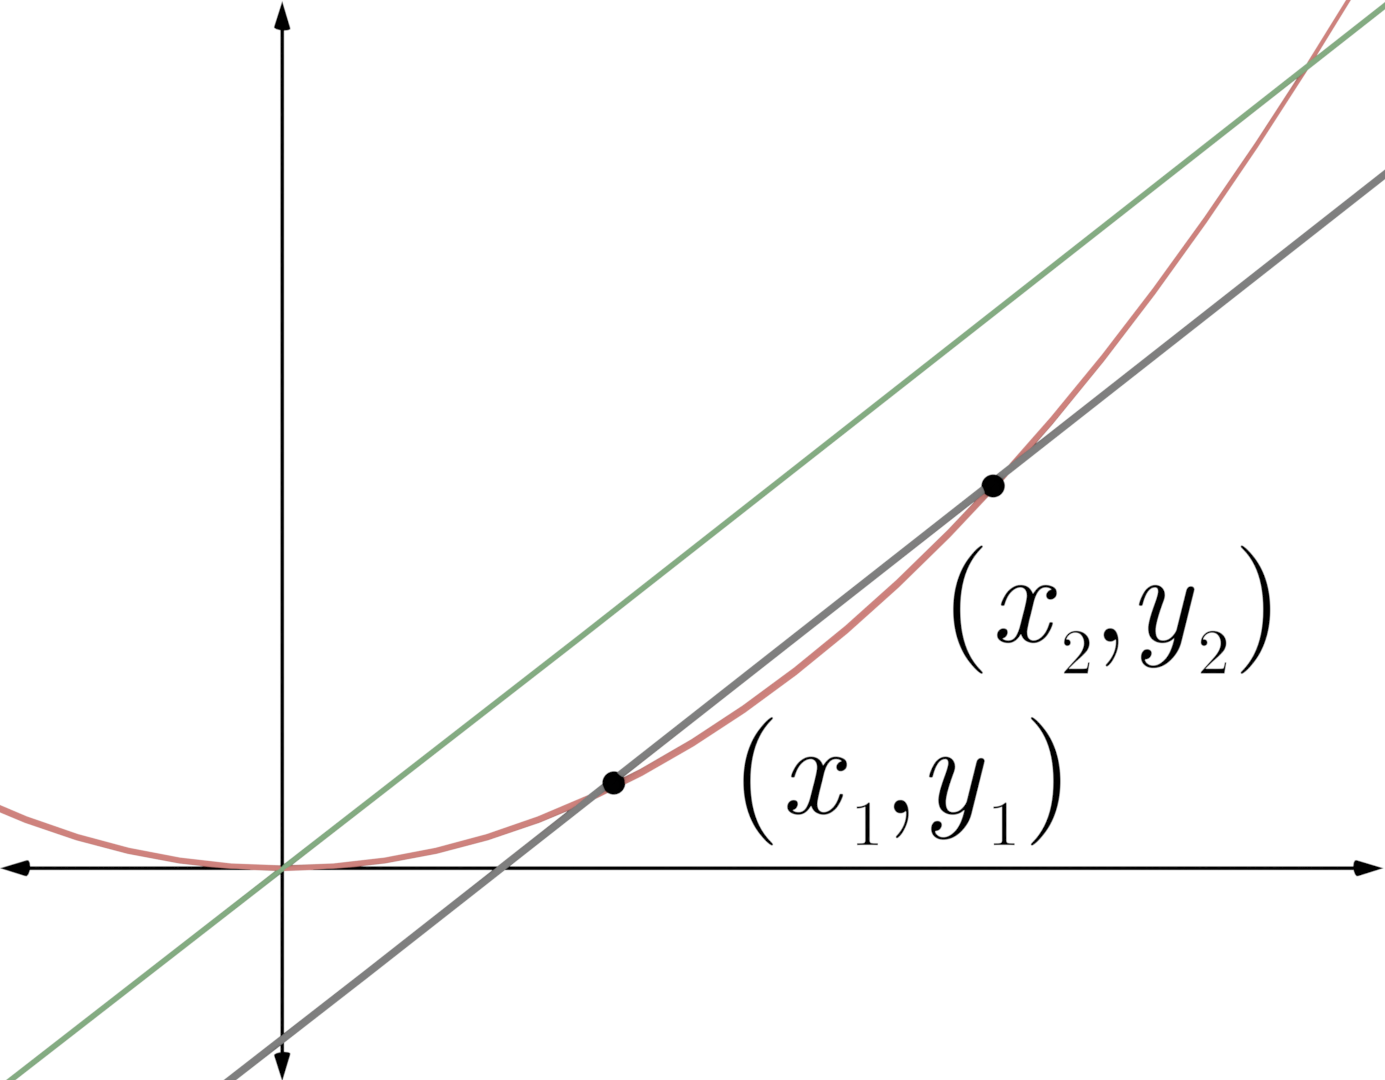
\includegraphics[width=0.57\linewidth]{Blender/ParabolaLineIntegration-ShellXY12-f2_0001.png}
  \caption{Determination of a shell's height.}
  \label{fig:shell2}
\end{figure}\par
Equipped with the four variables ($x_1$, $x_2$, $y_1$, and $y_2$) that it requires, use the distance formula$$d=\sqrt{\left(x_2-x_1\right)^2+\left(y_2-y_1\right)^2}$$to find the height of a shell as a function of $c$ as follows. Note that $h$ is substituted for $d$ because the distance given by the formula is the height of a shell.
\begin{align*}
h &= \sqrt{\left(\frac{b+\sqrt{b^2+4ac}}{2a}-\frac{b-\sqrt{b^2+4ac}}{2a}\right)^2+\left(\frac{b^2+2ac+b\sqrt{b^2+4ac}}{2a}-\frac{b^2+2ac-b\sqrt{b^2+4ac}}{2a}\right)^2}\\
   &= \sqrt{\left(\frac{2\sqrt{b^2+4ac}}{2a}\right)^2+\left(\frac{2b\sqrt{b^2+4ac}}{2a}\right)^2}\\
   &= \sqrt{\left(\frac{b^2+4ac}{a^2}\right)+\left(\frac{b^2\left(b^2+4ac\right)}{a^2}\right)}\\
   &= \sqrt{\frac{\left(1+b^2\right)\left(b^2+4ac\right)}{a^2}}\tag{6}
\end{align*}\par
With both the $r$ and the $h$ (equations 5 and 6, respectively) of the lateral area formula, $2\pi rh$, the only quantities left to determine are the bounds on the interval on which $c$ varies since it is necessary to integrate with respect to $c$. One bound is $0$ since the shell with the maximum height has a radius of $0$. However, the bound when the shell has maximum radius and a height of $0$ is more troublesome to determine. That being said, the key lies in the equations for $x_1$ and $x_2$, restated below for convenience.
\begin{align*}
x_1 &= \frac{b-\sqrt{b^2+4ac}}{2a} & x_2=\frac{b+\sqrt{b^2+4ac}}{2a}
\end{align*}\par
The variables, as seen in Figure \ref{fig:shell2}, are the intercepts of $y=bx+c$ and $y=ax^2$. However, when $h=0$, the two points are one and the same. In other words,
\begin{align*}
x_1 &= x_2\\
\frac{b-\sqrt{b^2+4ac}}{2a} &= \frac{b+\sqrt{b^2+4ac}}{2a}\\
b-\sqrt{b^2+4ac} &= b+\sqrt{b^2+4ac}\\
0 &= 2\sqrt{b^2+4ac}\\
   &= b^2+4ac\\
c &= \frac{-b^2}{4a}\tag{7}
\end{align*}
Therefore, $c$ varies on the interval $\left[\frac{-b^2}{4a},0\right]$.\par
Though it is possible to integrate at this point, a change of variable can eliminate the need for the absolute value in equation 5. Define$$w=-\frac{c}{\sqrt{1+b^2}}$$which keeps $w$ in the positive realm even as $c$ varies, making $|c|$ in equation 5 unnecessary. By plugging the bounds of the interval into the definition of $w$, generate the new interval $\left[0,\frac{b^2}{4a\sqrt{1+b^2}}\right]$. Finally, integrate. The volume equation is$$V=\int_0^{\frac{b^2}{4a\sqrt{1+b^2}}}2\pi\left(w\right)\left(\sqrt{\frac{\left(1+b^2\right)\left(b^2+4a\left(-w\sqrt{1+b^2}\right)\right)}{a^2}}\right)dw$$which can be simplified as follows.\par

\begin{align*}
V &= \int_0^{\frac{b^2}{4a\sqrt{1+b^2}}}2\pi\left(w\right)\left(\sqrt{\frac{\left(1+b^2\right)\left(b^2+4a\left(-w\sqrt{1+b^2}\right)\right)}{a^2}}\right)dw\\
   &= \int_0^{\frac{b^2}{4a\sqrt{1+b^2}}}2\pi w\sqrt{\frac{\left(1+b^2\right)\left(b^2-4a\sqrt{1+b^2}w\right)}{a^2}}\ dw\\
   &= \int_0^{\frac{b^2}{4a\sqrt{1+b^2}}}2\pi w\sqrt{\frac{\left(1+b^2\right)}{a^2}}\sqrt{b^2-4a\sqrt{1+b^2}w}\ dw\\
   &= 2\pi\sqrt{\frac{\left(1+b^2\right)}{a^2}}\int_0^{\frac{b^2}{4a\sqrt{1+b^2}}}\sqrt{b^2-4a\sqrt{1+b^2}w}\times w\ dw\tag{8}
\end{align*}
At this point, use the substitution,$$t=b^2-4a\sqrt{1+b^2}w$$to allow the radical to be integrated. Likewise,$$w=\frac{b^2-t}{4a\sqrt{1+b^2}}$$and$$dw=\frac{dt}{-4a\sqrt{1+b^2}}$$These substitutions allow equation 8 to be rewritten in terms of $t$, as shown below$$V=2\pi\sqrt{\frac{\left(1+b^2\right)}{a^2}}\int_0^{\frac{b^2}{4a\sqrt{1+b^2}}}\sqrt{t}\times\frac{b^2-t}{4a\sqrt{1+b^2}}\times\frac{dt}{-4a\sqrt{1+b^2}}$$This equation makes it much easier to finish the simplification, as follows.
\begin{align*}
V &= 2\pi\sqrt{\frac{\left(1+b^2\right)}{a^2}}\int_0^{\frac{b^2}{4a\sqrt{1+b^2}}}\sqrt{t}\times\frac{b^2-t}{4a\sqrt{1+b^2}}\times\frac{dt}{-4a\sqrt{1+b^2}}\\
   &= \frac{2\pi\sqrt{\frac{\left(1+b^2\right)}{a^2}}}{\left(4a\sqrt{1+b^2}\right)^2}\int_0^{\frac{b^2}{4a\sqrt{1+b^2}}}b^2\sqrt{t}-t\sqrt{t}\ dt\\
   &= \frac{2\pi\sqrt{\frac{\left(1+b^2\right)}{a^2}}}{16a^2\left(1+b^2\right)}\left(b^2\int_0^{\frac{b^2}{4a\sqrt{1+b^2}}}\sqrt{t}\ dt-\int_0^{\frac{b^2}{4a\sqrt{1+b^2}}}t^{\frac{3}{2}}\ dt\right)\\
   &= \frac{\pi}{8a^2}\sqrt{\frac{1}{a^2\left(1+b^2\right)}}\left(b^2\left[\frac{2t^{\frac{3}{2}}}{3}\right]_0^{\frac{b^2}{4a\sqrt{1+b^2}}}-\left[\frac{2t^{\frac{5}{2}}}{5}\right]_0^{\frac{b^2}{4a\sqrt{1+b^2}}}\right)\\
   &= \frac{\pi}{8a^3}\sqrt{\frac{1}{1+b^2}}\left(b^2\left[\frac{2\left(b^2-4a\sqrt{1+b^2}w\right)^{\frac{3}{2}}}{3}\right]_0^{\frac{b^2}{4a\sqrt{1+b^2}}}-\left[\frac{2\left(b^2-4a\sqrt{1+b^2}w\right)^{\frac{5}{2}}}{5}\right]_0^{\frac{b^2}{4a\sqrt{1+b^2}}}\right)
\end{align*}
\begin{align*}
V &= \frac{\pi}{8a^3}\sqrt{\frac{1}{1+b^2}}\left(b^2\left[\frac{2\left(b^2-4a\sqrt{1+b^2}\left(\frac{b^2}{4a\sqrt{1+b^2}}\right)\right)^{\frac{3}{2}}}{3}-\frac{2\left(b^2-4a\sqrt{1+b^2}\left(0\right)\right)^{\frac{3}{2}}}{3}\right]\right.\\
   &\hspace{16em} \left.-\left[\frac{2\left(b^2-4a\sqrt{1+b^2}\left(\frac{b^2}{4a\sqrt{1+b^2}}\right)\right)^{\frac{5}{2}}}{5}-\frac{2\left(b^2-4a\sqrt{1+b^2}\left(0\right)\right)^{\frac{5}{2}}}{5}\right]\right)\\
   &= \frac{\pi}{8a^3}\sqrt{\frac{1}{1+b^2}}\left(b^2\left[0-\frac{2\left(b^2\right)^{\frac{3}{2}}}{3}\right]-\left[0-\frac{2\left(b^2\right)^{\frac{5}{2}}}{5}\right]\right)\\
   &= \frac{\pi}{8a^3}\sqrt{\frac{1}{1+b^2}}\left(b^2\left[\frac{2b^3}{3}\right]-\left[\frac{2b^5}{5}\right]\right)\\
   &= \frac{\pi}{8a^3}\sqrt{\frac{1}{1+b^2}}\left(\frac{10b^5}{15}-\frac{6b^5}{15}\right)\\
   &= \frac{\pi}{8a^3}\sqrt{\frac{1}{1+b^2}}\left(\frac{4b^5}{15}\right)\\
   &= \frac{\pi b^5}{30a^3}\times\frac{\sqrt{1}}{\sqrt{1+b^2}}\\
   &= \frac{\pi b^5}{30a^3\sqrt{1+b^2}}\tag{9}
\end{align*}\par
\begin{flushright}
\textbf{Q.E.D.}
\end{flushright}

\subsection{Summary}
Though the algebra is more dense in the shell method than the cone method, it is still a valid way of finding the volume of the class of solids of revolution created by rotating the parabola, $y=ax^2$, about the line, $y=bx$. Furthermore, one benefit of it, as mentioned before, is that it generally takes less time to conceive, as it is a widely known and used technique. I was aware of the shell method before I began to consider this specific problem, but it was CopyPasteIt of Mathematics Stack Exchange in his answer \cite{BIB:shell} to my related question \cite{BIB:disk2} that suitably modified it to suit my needs.\par
However, the modifications are lengthy, as this procedure requires some major algebraic derivations as well as multiple changes of variable to make the integration possible in addition to the same knowledge of trigonometry as the cone method.\par
The next and last method is the most challenging --- it is a variation of the Disk Method.
\newpage

\section{Disk Method}
\subsection{Introduction}

\begin{figure}[h!]
  \centering
  \begin{subfigure}[b]{0.4\linewidth}
    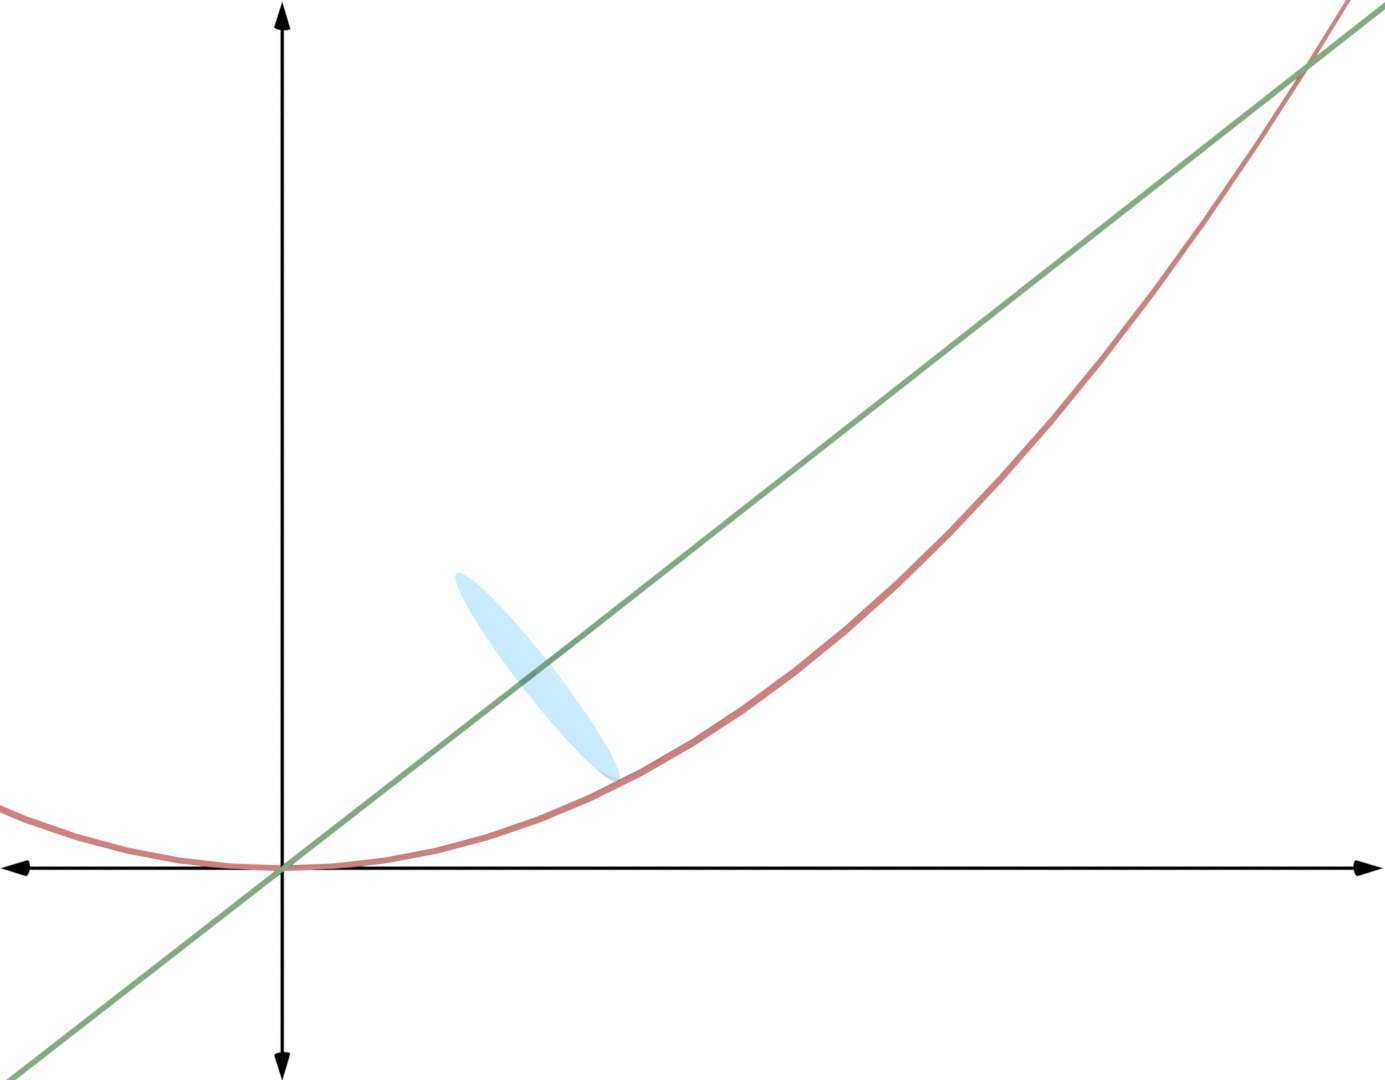
\includegraphics[width=\linewidth]{Blender/ParabolaLineIntegration-DiskDisk1-f2_0001.png}
    \caption{A disk.}
    \label{fig:diska}
  \end{subfigure}
  \begin{subfigure}[b]{0.4\linewidth}
    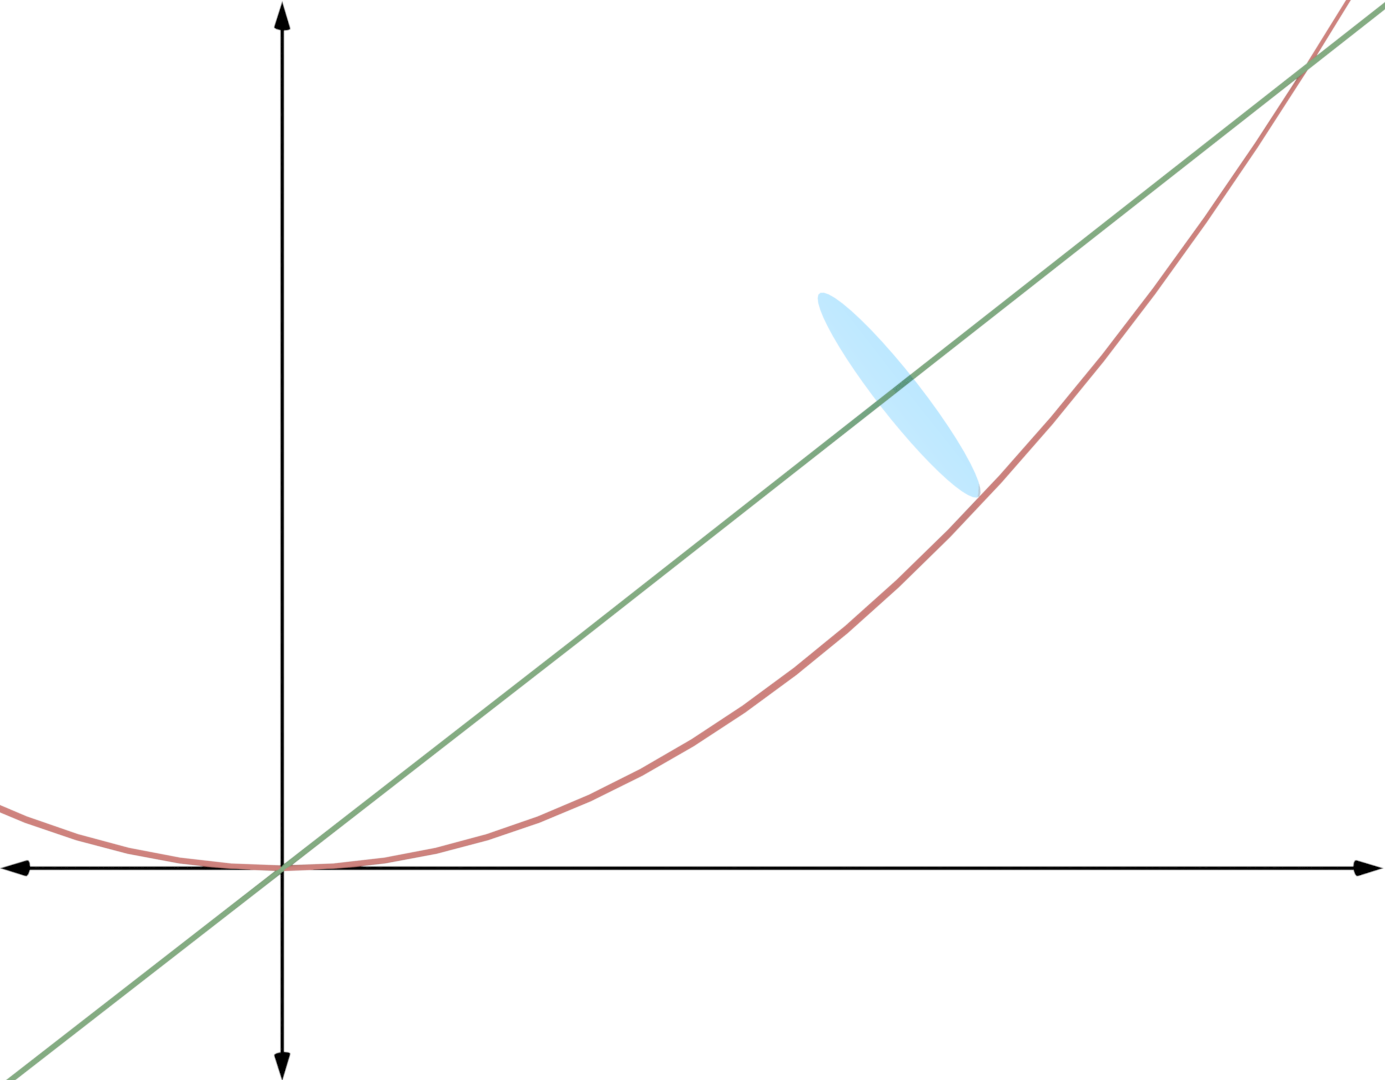
\includegraphics[width=\linewidth]{Blender/ParabolaLineIntegration-DiskDisk2-f2_0001.png}
    \caption{Another disk.}
    \label{fig:diskb}
  \end{subfigure}
  \caption{Formation of the disks.}
  \label{fig:disk1}
\end{figure}

This is the second of the two commonly taught methods of integrating to find volume. It utilizes a circle (disk) passing through the solid of revolution along the axis, growing and shrinking as it goes. The beauty of this method is that while both the shell and cone methods involved deriving two constants as functions, the disk method only requires the radius ($A=\pi r^2$). The difficulty is doing so can require a very lengthy derivation. If the axis of the solid of revolution is one of the literal $x$ or $y$ axes, then the radius is easy to find (it's either $f(x)$ or the inverse of $f(x)$). When the axis is not one of these, as in this case where it is given by the line $y=bx$, then the other function ($y=ax^2$, in this case) must be rotated an amount of degrees that varies with $b$.\par
This method requires the most setup to generate the eventual integrable equation. To begin with, investigate several methods of achieving this kind of rotation and settle on the easiest method that remains within the scope of this paper. Next, determine to what extent $y=ax^2$ must be rotated when the axis has slope $b$. Rotate $y=ax^2$ after this determination. The rotated function (on an interval) will give the radius of the solid of revolution. Integrate this function.

\subsection{Derivation} \label{deriv3}
\subsubsection{An Investigation of the Rotation of Conic Sections}
\paragraph{Matrices} The best, simplest way\footnote{Of which I am aware.} to rotate a conic section such as $y=ax^2$ uses rotation matrices. For example, Ennar of Mathematics Stack Exchange rotated the general parabola, $y=x^2$, (or, as he put it, $1x^2+0xy+0y^2+0x-1y+0=0$) clockwise by 45 degrees through the simplification \cite{BIB:disk1} of the following equation.
$$\begin{pmatrix} x & y & 1 \end{pmatrix}\begin{pmatrix} \cos \frac\pi4& -\sin\frac\pi4 & 0\\ \sin\frac\pi4 & \cos\frac\pi4 & 0\\ 0 & 0 & 1\end{pmatrix}^\tau\begin{pmatrix} 1 & 0 & 0\\ 0 & 0 & -1/2\\ 0 & -1/2 & 0\end{pmatrix}\begin{pmatrix} \cos \frac\pi4& -\sin\frac\pi4& 0\\ \sin\frac\pi4 & \cos\frac\pi4 & 0\\ 0 & 0 & 1\end{pmatrix}\begin{pmatrix} x\\ y\\ 1 \end{pmatrix}=0$$
Needless to say, this linear algebra is beyond the scope of this calculus paper.

\paragraph{Perpendicular} The second way (the most complicated) involves constructing a perpendicular to the axis that glides along the interval, $x\in\left[0,\frac{b}{a}\right]$. Find the coordinates of the points where the perpendicular intersects the axis and the conic section as a function of $x$ and use the distance formula. Finally, dilate the function by the distance between the two points of intersection of the conic and the axis. This was the method I proposed in the first half of my question \cite{BIB:disk2} to Mathematics Stack Exchange.

\paragraph{Focus/Directrix} The third way (the algebraically simplest\footnote{There could be a simpler way of which I am unaware.}) relies on conversion to and from the focus/directrix and Cartesian definitions of a conic section. As in sections \ref{deriv1} and \ref{deriv2}, begin by finding $\theta$ as a function of $b$. Next, find the focus and directrix of $y=ax^2$ as a function of $a$. Then, rotate the focus and directrix $\theta$ degrees using trigonometric functions. After that, determine the parabola from the new focus and directrix. Finally, solve for $y$, reflect the bottom half of it over the x-axis (so that the radius is positive), and integrate on an interval. Note that this method is also more logically sound than using perpendiculars.

\subsubsection{Derivation}
\paragraph{THEOREM} The volume of the solid of revolution created by rotating the parabola, $y=ax^2$, about the line, $y=bx$, is $\frac{\pi b^5}{30a^3\sqrt{1+b^2}}$ where $a>0$ and $b>0$.\par
\smallskip
\paragraph{PROOF} Begin by determining the focus and directrix of $y=ax^2$ as a function of $a$. Refer to Figure \ref{fig:disk2} throughout the following process. Let's define the variables in Figure \ref{fig:disk2}. $d_1$ is the distance from the directrix to a point on the parabola, $\left(x,y\right)$ or $\left(x,f(x)\right)$ or $\left(x,ax^2\right)$. $d_2$ is the distance from the focus to $\left(x,ax^2\right)$. Lastly, $y$ is the y-coordinate of the focus and of the constant in the equation of the directrix, $y=c$.\par
According to the focus/directrix definition of a conic section,$$d_1=ed_2$$ where $e$ is the eccentricity. In a parabola, $e=1$, so$$d_1=d_2$$This is the key to finding the focus and directrix. Note that this is also why the focus and directrix share a y-value --- according to $d_1=d_2$, they must be equidistant from $(0,0)$, a point on the parabola.

\begin{figure}[h!]
  \centering
  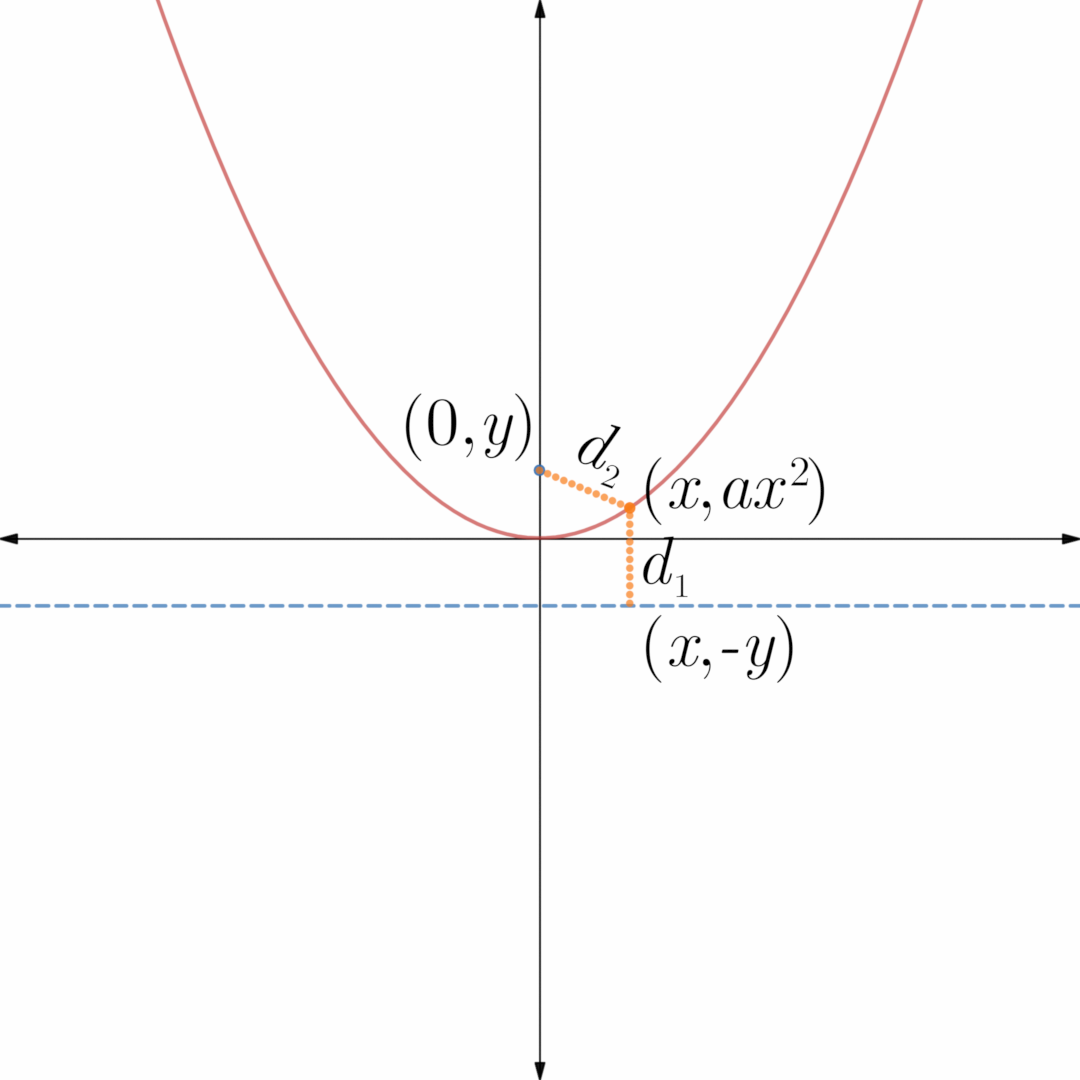
\includegraphics[width=0.6\linewidth]{Blender/ParabolaLineIntegration-DiskFD1-f2_0001.png}
  \caption{Focus and directrix of $y=ax^2$ before rotation.}
  \label{fig:disk2}
\end{figure}\par

To determine the focus, use the distance formula to define $d_1$ and $d_2$ in terms of $x$, $y$, and $a$, set the new equations equal to each other, and simplify.

\begin{align*}
d_1 &= \sqrt{\left(x-x\right)^2+\left(ax^2-(-y)\right)^2}\\
       &= \sqrt{0+\left(ax^2+y\right)^2}\\
       &= \sqrt{\left(ax^2+y\right)^2}
\end{align*}
\begin{align*}
d_2 &= \sqrt{\left(x-0\right)^2+\left(ax^2-y\right)^2}\\
       &= \sqrt{x^2+\left(ax^2-y\right)^2}\\
\end{align*}
\begin{align*}
d_1 &= d_2\\
\sqrt{\left(ax^2+y\right)^2} &= \sqrt{x^2+\left(ax^2-y\right)^2}\\
\left(ax^2+y\right)^2 &= x^2+\left(ax^2-y\right)^2\\
a^2x^4+2ax^2y+y^2 &= x^2+\left(a^2x^4-2ax^2y+y^2\right)\\
4ax^2y &= x^2\\
y &= \frac{1}{4a}\tag{10}
\end{align*}\par

With the y-coordinate of the focus given by equation 10, it becomes clear that the focus of $y=ax^2$ is at $\left(0,\frac{1}{4a}\right)$. To determine the directrix, reflect the y-coordinate of the focus over the x-axis and express it as an equation in the form $y=c$. In other words, the directrix of the parabola, $y=ax^2$ is given by $y=-\frac{1}{4a}$.

\begin{figure}[h!]
  \centering
  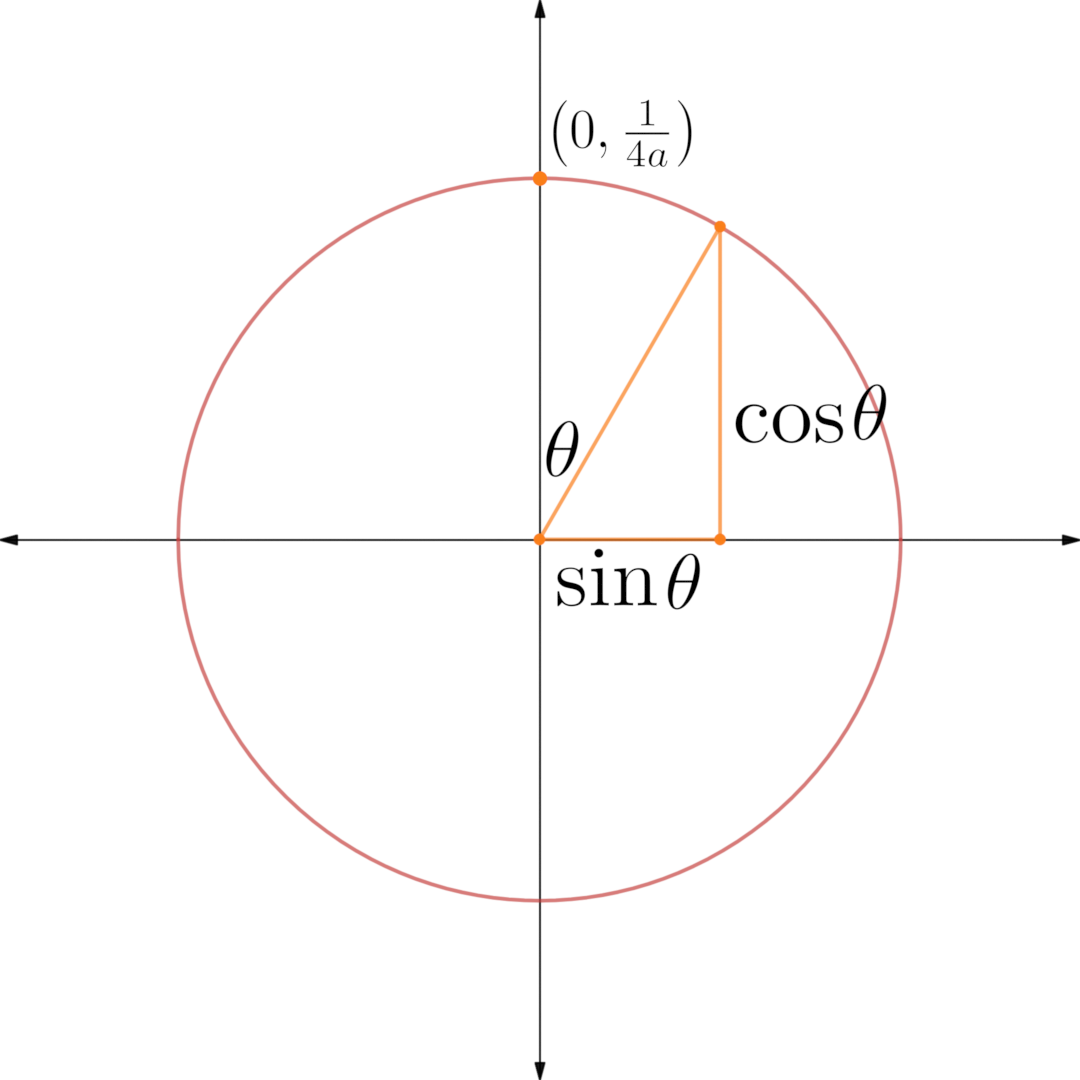
\includegraphics[width=0.54\linewidth]{Blender/ParabolaLineIntegration-DiskParameter-f_0001.png}
  \caption{Rotating the focus.}
  \label{fig:disk3}
\end{figure}\par

Before rotating the parabola, it is necessary to define $\theta$ in terms of $b$, as was done in both section \ref{deriv1} and \ref{deriv2}. The same refresher that was given in section \ref{deriv2} is listed below (refer to Figure \ref{fig:cone3} for a related visual).\par
The definition of tangent gives the following equation. Simplify, and solve for $\theta$.
\begin{align*}
\tan\theta &=\frac{bx}{x}=b\\
\theta       &= \tan^{-1}\left(b\right)
\end{align*}\par
Next, rotate the focus and directrix $\theta$ degrees about the origin. Begin with the focus. To accomplish this rotation, regard the coordinate, $\left(0,\frac{1}{4a}\right)$, as a point on a circle with radius, $r=\frac{1}{4a}$, defined by the parametrization,
\begin{align*}
x &= \frac{1}{4a}\sin\theta\\
y &= \frac{1}{4a}\cos\theta
\end{align*}
as seen in Figure \ref{fig:disk3}. As the reader can see, by plugging in $\theta=0^\circ$, the $x$ and $y$ coordinates come out as expected as $\left(0,\frac{1}{4a}\right)$. However, eliminating $\theta$ requires the substitution listed above in the refresher. Again, refer to Figure \ref{fig:cone3} for a related visual.

\begin{align*}
x &= \frac{1}{4a}\sin\left(\tan^{-1}(b)\right)\\
y &= \frac{1}{4a}\cos\left(\tan^{-1}(b)\right)\\
\vspace{1em}\\
x &= \frac{1}{4a}\times\frac{b}{\sqrt{1+b^2}}\\
y &= \frac{1}{4a}\times\frac{1}{\sqrt{1+b^2}}\\
\vspace{1em}\\
x &= \frac{b}{4a\sqrt{1+b^2}}\\
y &= \frac{1}{4a\sqrt{1+b^2}}
\end{align*}

Rotating the directrix is somewhat more complicated. It is necessary to reflect the rotated point, $\left(\frac{b}{4a\sqrt{1+b^2}},\frac{1}{4a\sqrt{1+b^2}}\right)$, over both the $x$ and $y$ axes. Then, define an equation in point-slope form that runs through the reflected, rotated point with a slope identical to that of the reflection of $y=bx$ over the y-axis (that is, a slope of $m=-b$). Therefore, the equation of the directrix is equation 11 below, simplified from the general point-slope form listed at the top of the series.

\begin{align*}
y-y_1 &= m\left(x-x_1\right)\\
y-\left(-\frac{1}{4a\sqrt{1+b^2}}\right) &= -b\left(x-\left(-\frac{b}{4a\sqrt{1+b^2}}\right)\right)\\
y+\frac{1}{4a\sqrt{1+b^2}} &= -bx-\frac{b^2}{4a\sqrt{1+b^2}}\\
y &= -bx-\frac{b^2+1}{4a\sqrt{1+b^2}}\tag{11}
\end{align*}

Now, we have all of the tools necessary to find the equation of the rotated parabola. Refer to Figure \ref{fig:disk4} throughout this derivation for a related visual.

\begin{figure}[h!]
  \centering
  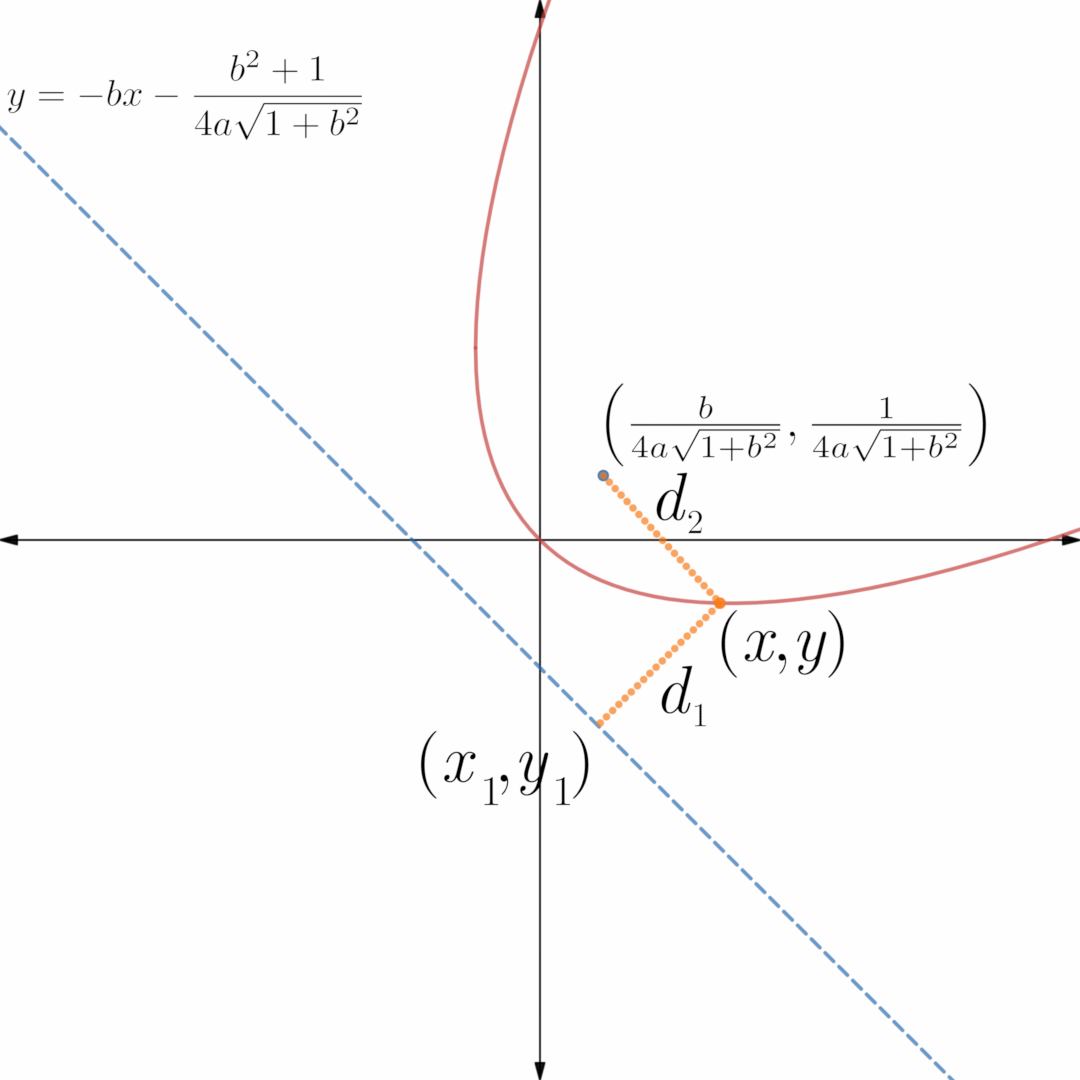
\includegraphics[width=0.6\linewidth]{Blender/ParabolaLineIntegration-DiskFD2-f2_0001.png}
  \caption{Focus and directrix of $y=ax^2$ after rotation.}
  \label{fig:disk4}
\end{figure}

Once again, $d_1$ is more difficult to define in terms of $x$, $y$, $a$, and $b$. Before using the distance formula, it is necessary to find the coordinate, $\left(x_1,y_1\right)$, in terms of these constants and variables. Note that $\left(x_1,y_1\right)$ in Figure \ref{fig:disk4} plays the same role as $\left(x,-y\right)$ in Figure \ref{fig:disk2} i.e. the point where the perpendicular line segment to the directrix dropped from the moveable point along the function intersects the directrix. In fact, it is this perpendicular nature that ends up being the key to finding $x_1$ and $y_1$ as functions of $x$, $y$, $a$, and $b$. If a line in point-slope form is defined that passes through $(x,y)$ with slope $m=\frac{1}{b}$ (the negative reciprocal of the slope of the directrix), it will intersect the directrix at $\left(x_1,y_1\right)$. The line given by equation 12 below
\begin{align*}
y_1-y &= m\left(x_1-x\right)\\
y_1 &= \frac{1}{b}x_1-\frac{x}{b}+y\tag{12}
\end{align*}
has all of these characteristics, providing the second equation necessary for the system of equations,
\begin{align*}
y_1 &= \frac{1}{b}x_1-\frac{x}{b}+y\\
y_1 &= -bx_1-\frac{b^2+1}{4a\sqrt{1+b^2}}
\end{align*}
which is solved for $x_1$ below.
\begin{align*}
\frac{1}{b}x_1-\frac{x}{b}+y &= -bx_1-\frac{b^2+1}{4a\sqrt{1+b^2}}\\
\frac{1}{b}x_1+bx_1 &= \frac{x}{b}-y-\frac{b^2+1}{4a\sqrt{1+b^2}}\\
\frac{b^2+1}{b}x_1 &= \frac{x}{b}-y-\frac{b^2+1}{4a\sqrt{1+b^2}}\\
x_1 &= \frac{1}{b^2+1}x-\frac{b}{b^2+1}y-\frac{b}{4a\sqrt{1+b^2}}
\end{align*}
Given $x_1$, plug into equation 11 to find $y_1$, as follows.
\begin{align*}
y_1 &= -bx_1-\frac{b^2+1}{4a\sqrt{1+b^2}}\\
       &= -b\left(\frac{1}{b^2+1}x-\frac{b}{b^2+1}y-\frac{b}{4a\sqrt{1+b^2}}\right)-\frac{b^2+1}{4a\sqrt{1+b^2}}\\
       &= -\frac{b}{b^2+1}x+\frac{b^2}{b^2+1}y+\frac{b^2}{4a\sqrt{1+b^2}}-\frac{b^2+1}{4a\sqrt{1+b^2}}\\
       &= -\frac{b}{b^2+1}x+\frac{b^2}{b^2+1}y-\frac{1}{4a\sqrt{1+b^2}}
\end{align*}
With definitions for $x_1$ and $y_1$ (and, of course, $x$ and $y$ as themselves) in terms of $x$, $y$, $a$, and $b$, it is now possible to use the distance formula to find $d_1$ as follows.
\begin{align*}
d &= \sqrt{\left(x_2-x_1\right)^2+\left(y_2-y_1\right)^2}\\
d_1 &= \sqrt{\left(x-\left(\frac{1}{b^2+1}x-\frac{b}{b^2+1}y-\frac{b}{4a\sqrt{1+b^2}}\right)\right)^2+\left(y-\left(-\frac{b}{b^2+1}x+\frac{b^2}{b^2+1}y-\frac{1}{4a\sqrt{1+b^2}}\right)\right)^2}\\
       &= \sqrt{\left(\frac{b^2+1}{b^2+1}x-\frac{1}{b^2+1}x+\frac{b}{b^2+1}y+\frac{b}{4a\sqrt{1+b^2}}\right)^2+\left(\frac{b^2+1}{b^2+1}y+\frac{b}{b^2+1}x-\frac{b^2}{b^2+1}y+\frac{1}{4a\sqrt{1+b^2}}\right)^2}\\
       &= \sqrt{\left(\frac{b^2}{b^2+1}x+\frac{b}{b^2+1}y+\frac{b}{4a\sqrt{1+b^2}}\right)^2+\left(\frac{b}{b^2+1}x+\frac{1}{b^2+1}y+\frac{1}{4a\sqrt{1+b^2}}\right)^2}\\
       &= \sqrt{\left(\frac{b^2x+by}{b^2+1}+\frac{b}{4a\sqrt{1+b^2}}\right)^2+\left(\frac{bx+y}{b^2+1}+\frac{1}{4a\sqrt{1+b^2}}\right)^2}\tag{13}
\end{align*}

$d_2$ is fairly simple to find, if another look is taken at Figure \ref{fig:disk4}. Use the distance formula once again, as follows.
\begin{align*}
d &= \sqrt{\left(x_2-x_1\right)^2+\left(y_2-y_1\right)^2}\\
d_2 &= \sqrt{\left(x-\frac{b}{4a\sqrt{1+b^2}}\right)^2+\left(y-\frac{1}{4a\sqrt{1+b^2}}\right)^2}\tag{14}
\end{align*}

By setting equations 13 and 14 equal to each other (allowed since $d_1=d_2$), it is possible to obtain the equation of the final rotated parabola (which will give the radius of the teardrop shape as a function of $x$) upon simplification. The process is listed below.
\begin{align*}
d_1 &= d_2\\
\sqrt{\left(\frac{b^2x+by}{b^2+1}+\frac{b}{4a\sqrt{1+b^2}}\right)^2+\left(\frac{bx+y}{b^2+1}+\frac{1}{4a\sqrt{1+b^2}}\right)^2} &= \sqrt{\left(x-\frac{b}{4a\sqrt{1+b^2}}\right)^2+\left(y-\frac{1}{4a\sqrt{1+b^2}}\right)^2}\\
\left(\frac{b^2x+by}{b^2+1}+\frac{b}{4a\sqrt{1+b^2}}\right)^2+\left(\frac{bx+y}{b^2+1}+\frac{1}{4a\sqrt{1+b^2}}\right)^2 &= \left(x-\frac{b}{4a\sqrt{1+b^2}}\right)^2+\left(y-\frac{1}{4a\sqrt{1+b^2}}\right)^2\\
\end{align*}
For the sake of simplicity, use the following substitutions.
\begin{align*}
u &= \frac{bx+y}{b^2+1} &
v &= \frac{1}{4a\sqrt{1+b^2}}
\end{align*}
Finish the simplification.
\begin{align*}
(bu+bv)^2+(u+v)^2 &= (x-bv)^2+(y-v)^2\\
b^2(u^2+2uv+v^2)+(u^2+2uv+v^2) &= (x^2-2bvx+b^2v^2)+(y^2-2vy+v^2)\\
b^2u^2+2b^2uv+b^2v^2+u^2+2uv+v^2 &= x^2-2bvx+b^2v^2+y^2-2vy+v^2\\
b^2u^2+2b^2uv+u^2+2uv &= x^2-2bvx+y^2-2vy\\
(1+b^2)u^2+2v(b^2u+u) &= x^2+y^2-2v(bx+y)\\
(1+b^2)\left(\frac{bx+y}{b^2+1}\right)^2+2\left(\frac{1}{4a\sqrt{1+b^2}}\right)\left(b^2\left(\frac{bx+y}{b^2+1}\right)+\left(\frac{bx+y}{b^2+1}\right)\right) &= x^2+y^2-2\left(\frac{1}{4a\sqrt{1+b^2}}\right)(bx+y)\\
\frac{b^2x^2+2bxy+y^2}{b^2+1}+\frac{2b^3x+2b^2y+2bx+2y}{4a(b^2+1)\sqrt{1+b^2}} &= x^2+y^2-\frac{2bx+2y}{4a\sqrt{1+b^2}}\\
\frac{b^2x^2+2bxy+y^2}{b^2+1}+\frac{b^3x+b^2y+bx+y}{2a(b^2+1)\sqrt{1+b^2}} &= x^2+y^2-\frac{b^3x+b^2y+bx+y}{2a(b^2+1)\sqrt{1+b^2}}\\
\frac{b^2}{b^2+1}x^2+\frac{2b}{b^2+1}xy+\frac{1}{b^2+1}y^2+\frac{b^3+b}{a(b^2+1)\sqrt{1+b^2}}x+\frac{1}{a\sqrt{1+b^2}}y &= \frac{b^2+1}{b^2+1}x^2+\frac{b^2+1}{b^2+1}y^2\\
-\frac{1}{b^2+1}x^2+\frac{2b}{b^2+1}xy-\frac{b^2}{b^2+1}y^2+\frac{b}{a\sqrt{1+b^2}}x+\frac{1}{a\sqrt{1+b^2}}y &= 0\\
\frac{1}{b^2+1}x^2-\frac{2b}{b^2+1}xy+\frac{b^2}{b^2+1}y^2-\frac{b}{a\sqrt{1+b^2}}x-\frac{1}{a\sqrt{1+b^2}}y &= 0\tag{15}
\end{align*}

Since there is no such thing as implicit integration, it is necessary to solve equation 15 for $y$. If equation 15 is regarded as a quadratic equation in $y$, it is possible to solve it using the quadratic formula, as follows.
\begin{align*}
0 &= \left(\frac{b^2}{b^2+1}\right)y^2+\left(-\frac{2bx}{b^2+1}-\frac{1}{a\sqrt{1+b^2}}\right)y+\left(\frac{x^2}{b^2+1}-\frac{bx}{a\sqrt{1+b^2}}\right)\\
y &= \frac{-\left(-\frac{2bx}{b^2+1}-\frac{1}{a\sqrt{1+b^2}}\right)\pm\sqrt{\left(-\frac{2bx}{b^2+1}-\frac{1}{a\sqrt{1+b^2}}\right)^2-4\left(\frac{b^2}{b^2+1}\right)\left(\frac{x^2}{b^2+1}-\frac{bx}{a\sqrt{1+b^2}}\right)}}{2\left(\frac{b^2}{b^2+1}\right)}\\
   &= \frac{\frac{2bx}{b^2+1}+\frac{1}{a\sqrt{1+b^2}}\pm\sqrt{\left(\frac{2bx}{b^2+1}+\frac{1}{a\sqrt{1+b^2}}\right)^2-\left(\frac{4b^2}{b^2+1}\right)\left(\frac{x^2}{b^2+1}-\frac{bx}{a\sqrt{1+b^2}}\right)}}{\frac{2b^2}{b^2+1}}\\
   &= \frac{x}{b}+\frac{\sqrt{1+b^2}}{2ab^2}\pm\frac{b^2+1}{2b^2}\sqrt{\left(\frac{4b^2x^2}{(b^2+1)^2}+\frac{4bx}{a(1+b^2)\sqrt{1+b^2}}+\frac{1}{a^2+a^2b^2}\right)-\left(\frac{4b^2x^2}{(b^2+1)^2}-\frac{4b^3x}{a(b^2+1)\sqrt{1+b^2}}\right)}\\
   &= \frac{x}{b}+\frac{\sqrt{1+b^2}}{2ab^2}\pm\frac{b^2+1}{2b^2}\sqrt{\frac{1}{a^2+a^2b^2}+\frac{4bx}{a(1+b^2)\sqrt{1+b^2}}+\frac{4b^3x}{a(b^2+1)\sqrt{1+b^2}}}\\
   &= \frac{x}{b}+\frac{\sqrt{1+b^2}}{2ab^2}\pm\frac{b^2+1}{2b^2}\sqrt{\frac{1}{a^2+a^2b^2}+\frac{4b^3x+4bx}{a(b^2+1)\sqrt{1+b^2}}}\\
   &= \frac{x}{b}+\frac{\sqrt{1+b^2}}{2ab^2}\pm\frac{b^2+1}{2b^2}\sqrt{\frac{1}{a^2+a^2b^2}+\frac{4b}{a\sqrt{1+b^2}}x}\\
   &= \frac{x}{b}+\frac{\sqrt{1+b^2}}{2ab^2}\pm\frac{b^2+1}{2b^2}\sqrt{\frac{4abx\sqrt{1+b^2}+1}{a^2+a^2b^2}}\\
   &= \frac{x}{b}+\frac{\sqrt{1+b^2}}{2ab^2}\pm\frac{(b^2+1)\sqrt{4abx\sqrt{1+b^2}+1}}{2ab^2\sqrt{1+b^2}}\\
   &= \frac{1}{b}x+\frac{\sqrt{1+b^2}}{2ab^2}\pm\frac{\sqrt{1+b^2}}{2ab^2}\sqrt{4abx\sqrt{1+b^2}+1}
\end{align*}

Finally, the last equation is integrable with only the slight modification that the $\pm$ sign must become a $-$ sign since the necessary half of the parabola is the one that intersects the x-axis and the entire right side must be multiplied by $-1$ since the radius is always positive. With these changes, the radius of the solid of revolution as a function of $x$ along the axis, $y=bx$ is
\begin{equation*}
r=-\frac{1}{b}x-\frac{\sqrt{1+b^2}}{2ab^2}+\frac{\sqrt{1+b^2}}{2ab^2}\sqrt{4abx\sqrt{1+b^2}+1}\tag{16}
\end{equation*}
The only thing left to determine is the interval on which to integrate. Once again, the left bound is obviously $0$. The right bound is the distance along the axis, $y=bx$, between its two intercepts with the parabola, $y=ax^2$. Since (as was proven in section \ref{deriv1}) the x-coordinate of the rightmost intercept of the parabola and the axis is $\frac{b}{a}$, the y-coordinate is $y=bx=b\left(\frac{b}{a}\right)=\frac{b^2}{a}$. Then, by the distance formula, the right bound is as follows. Note that $B_R$ is used to denote the right bound.
\begin{align*}
d &= \sqrt{\left(x_2-x_1\right)^2+\left(y_2-y_1\right)^2}\\
B_R &= \sqrt{\left(\frac{b}{a}-0\right)^2+\left(\frac{b^2}{a}-0\right)^2}\\
        &= \sqrt{\frac{b^2}{a^2}+\frac{b^4}{a^2}}\\
        &= \sqrt{\frac{b^2(1+b^2)}{a^2}}\\
        &= \frac{b}{a}\sqrt{1+b^2}\tag{17}
\end{align*}
According to equation 17, it is necessary to integrate on the interval, $\left[0,\frac{b}{a}\sqrt{1+b^2}\right]$. At last, it is possible to set up the volume equation
\begin{equation*}
V=\int_0^{\frac{b}{a}\sqrt{1+b^2}}\pi\left(-\frac{1}{b}x-\frac{\sqrt{1+b^2}}{2ab^2}+\frac{\sqrt{1+b^2}}{2ab^2}\sqrt{4abx\sqrt{1+b^2}+1}\right)^2dx\tag{18}
\end{equation*}
which, suffice to say, does indeed simplify to the very same
\begin{equation*}
V=\frac{\pi b^5}{30a^3\sqrt{1+b^2}}\tag{19}
\end{equation*}
Unfortunately, while the algebra of the final step in sections \ref{deriv1} and \ref{deriv2} was relatively comprehensible, the simplification of equation 18 to equation 19 is far too dense to be effectively or realistically transcribed here. To those who remain curious, any sufficiently powerful integral calculator can confirm the transition (I recommend Desmos --- I have constructed the scenario \textcolor{blue}{\underline{\emph{\href{https://www.desmos.com/calculator/ssaa0mva1t}{here}}}}).
\begin{flushright}
\textbf{Q.E.D.}
\end{flushright}

\subsection{Summary}
This method, as demonstrated by section \ref{deriv3}'s length, the complexity of its calculations, and the exhaustive nature of the transition from equation 18-19, is by far the most complicated. That being said, it is still perfectly mathematically viable and does provide the same answer as the cone and shell methods in the end. Furthermore, this method takes the least time to conceive. In fact, it is a variation of this method (using the perpendicular technique to rotate the parabola) that I developed and initially used in my question \cite{BIB:disk2} to Mathematics Stack Exchange.\par
Though this procedure has the upsides of being my own and of being valid, it is a most arduous process. The algebraic derivations, such as the one that begins after equation 11 and culminates in equation 16, are extremely intense. The calculus in equation 18, besides requiring substitutions, necessitates an all-out expansion and collection of like terms to reduce to equation 19 i.e. there is no way\footnote{I have not found such a process.} to solve it in a few easy steps.\par
Though there may be more methods to find the volume of the class of solids of revolution created by rotating the parabola, $y=ax^2$, about the axis, $y=bx$, this concludes those that will be explored in this paper.
\newpage
\setcounter{secnumdepth}{0}

\bibliography{SORVolumes}
\bibliographystyle{ieeetr}
All figures are my own designs, created in Blender 3D with style influenced by Desmos.

\end{document}